% This is "sig-alternate.tex" V2.0 May 2012
% This file should be compiled with V2.5 of "sig-alternate.cls" May 2012
%
% This example file demonstrates the use of the 'sig-alternate.cls'
% V2.5 LaTeX2e document class file. It is for those submitting
% articles to ACM Conference Proceedings WHO DO NOT WISH TO
% STRICTLY ADHERE TO THE SIGS (PUBS-BOARD-ENDORSED) STYLE.
% The 'sig-alternate.cls' file will produce a similar-looking,
% albeit, 'tighter' paper resulting in, invariably, fewer pages.
%
% ----------------------------------------------------------------------------------------------------------------
% This .tex file (and associated .cls V2.5) produces:
%       1) The Permission Statement
%       2) The Conference (location) Info information
%       3) The Copyright Line with ACM data
%       4) NO page numbers
%
% as against the acm_proc_article-sp.cls file which
% DOES NOT produce 1) thru' 3) above.
%
% Using 'sig-alternate.cls' you have control, however, from within
% the source .tex file, over both the CopyrightYear
% (defaulted to 200X) and the ACM Copyright Data
% (defaulted to X-XXXXX-XX-X/XX/XX).
% e.g.
% \CopyrightYear{2007} will cause 2007 to appear in the copyright line.
% \crdata{0-12345-67-8/90/12} will cause 0-12345-67-8/90/12 to appear in the copyright line.
%
% ---------------------------------------------------------------------------------------------------------------
% This .tex source is an example which *does* use
% the .bib file (from which the .bbl file % is produced).
% REMEMBER HOWEVER: After having produced the .bbl file,
% and prior to final submission, you *NEED* to 'insert'
% your .bbl file into your source .tex file so as to provide
% ONE 'self-contained' source file.
%
% ================= IF YOU HAVE QUESTIONS =======================
% Questions regarding the SIGS styles, SIGS policies and
% procedures, Conferences etc. should be sent to
% Adrienne Griscti (griscti@acm.org)
%
% Technical questions _only_ to
% Gerald Murray (murray@hq.acm.org)
% ===============================================================
%
% For tracking purposes - this is V2.0 - May 2012

\documentclass{sig-alternate}
\usepackage{tikz}
  \def\firstcircle{(90:1.75cm) circle (2.5cm)}
  \def\secondcircle{(210:1.75cm) circle (2.5cm)}
  \def\thirdcircle{(330:1.75cm) circle (2.5cm)} 
\usepackage{comment}
\usepackage{cite}
\usepackage[shortlabels]{enumitem} 
\usepackage{amsmath}
\usepackage{url}
\usepackage{balance}
\newcommand{\bi}{\begin{itemize}[leftmargin=0.4cm]}
\newcommand{\ei}{\end{itemize}}
\newcommand{\be}{\begin{enumerate}}
\newcommand{\ee}{\end{enumerate}}
\newcommand{\tion}[1]{\S\ref{sect:#1}}
\newcommand{\fig}[1]{Figure~\ref{fig:#1}}
\newcommand{\eq}[1]{Equation~\ref{eq:#1}}
\setlist{nolistsep,leftmargin=5mm}
%\usepackage[pdftex]{graphicx}
\newcommand{\Sample}{{\bf SAMPLE}}
\newcommand{\PEEKING}{{\bf PEEKING2}}
\usepackage{picture}
\usepackage{colortbl}
\usepackage[table]{xcolor}
\usepackage{listings}
%\usepackage[margin=1in]{geometry}

\definecolor{lightgray}{gray}{0.8}
\definecolor{darkgray}{gray}{0.6}
\usepackage{tabu}

%XXX also note in 2.1 the rpevalnce of model-based methds

\definecolor{Gray}{gray}{0.95}
\definecolor{LightGray}{gray}{0.975}

\lstset{
    language=Python,
    basicstyle=\ttfamily\fontsize{2.4mm}{0.8em}\selectfont,
    breaklines=true,
    prebreak=\raisebox{0ex}[0ex][0ex]{\ensuremath{\hookleftarrow}},
    frame=tlrb,
    showtabs=false,
    showspaces=false,
    showstringspaces=false,
    %backgroundcolor=\color{Gray},
    keywordstyle=\bfseries,
    emph={COCONUT,GUESSES,ASSESS,COCOMO2,PEEKING2,SAMPLE,WHERE,RIG}, emphstyle=\bfseries\color{Blue},
    stringstyle=\color{green!50!black},
    commentstyle=\color{red}\itshape,
    %numbers=none,
    captionpos=t,
    numberstyle=\bfseries\color{red},
    escapeinside={\%*}{*)}
}

\definecolor{darkgreen}{rgb}{0,0.3,0}

\usepackage[table]{xcolor}
\definecolor{Gray}{rgb}{0.88,1,1}
\definecolor{Gray}{gray}{0.85}
\definecolor{Blue}{RGB}{0,29,193}

\newcommand{\G}{\cellcolor{green}}
\newcommand{\Y}{\cellcolor{yellow}}

\newcommand{\quart}[4]{\begin{picture}(100,4)%1
{\color{black}\put(#3,2){\circle*{4}}\put(#1,2){\line(1,0){#2}}}\end{picture}}



\definecolor{MyDarkBlue}{rgb}{0,0.08,0.45} 
%\newenvironment{changed}{\par\color{MyDarkBlue}}{\par}
\newenvironment{changed}{\par}{\par}

%\newcommand{\ADD}[1]{\textcolor{MyDarkBlue}{{\bf #1}}}
\newcommand{\ADD}[1]{#1}
 


\usepackage{times}

\def\baselinestretch{1}


\setlist{nosep}

 \usepackage[font={small}]{caption, subfig}



\setlength{\abovecaptionskip}{1ex}
 \setlength{\belowcaptionskip}{1ex}
 
 \setlength{\floatsep}{1ex}
 \setlength{\textfloatsep}{1ex}
 \newcommand{\subparagraph}{} % defined before loading titlesec
\usepackage[compact,small]{titlesec}
\DeclareMathSizes{7}{7}{7}{7} 
%\renewcommand{\footnotesize}{\scriptsize}

\pagenumbering{arabic} 
\begin{document}  
%
% --- Author Metadata here ---
\conferenceinfo{FSE}{'15 Bergamo, Italy}
%\CopyrightYear{2007} % Allows default copyright year (20XX) to be over-ridden - IF NEED BE.
%\crdata{0-12345-67-8/90/01}  % Allows default copyright data (0-89791-88-6/97/05) to be over-ridden - IF NEED BE.
% --- End of Author Metadata ---


\title{On the Value of Parametric Software Effort Estimation}


%
% You need the command \numberofauthors to handle the 'placement
% and alignment' of the authors beneath the title.
%
% For aesthetic reasons, we recommend 'three authors at a time'
% i.e. three 'name/affiliation blocks' be placed beneath the title.
%
% NOTE: You are NOT restricted in how many 'rows' of
% "name/affiliations" may appear. We just ask that you restrict
% the number of 'columns' to three.
%
% Because of the available 'opening page real-estate'
% we ask you to refrain from putting more than six authors
% (two rows with three columns) beneath the article title.
% More than six makes the first-page appear very cluttered indeed.
%
% Use the \alignauthor commands to handle the names
% and affiliations for an 'aesthetic maximum' of six authors.
% Add names, affiliations, addresses for
% the seventh etc. author(s) as the argument for the
% \additionalauthors command.
% These 'additional authors' will be output/set for you
% without further effort on your part as the last section in
% the body of your article BEFORE References or any Appendices.

\numberofauthors{3} %  in this sample file, there are a *total*
% of EIGHT authors. SIX appear on the 'first-page' (for formatting
% reasons) and the remaining two appear in the \additionalauthors section.
%

\author{
% You can go ahead and credit any number of authors here,
% e.g. one 'row of three' or two rows (consisting of one row of three
% and a second row of one, two or three).
%
% The command \alignauthor (no curly braces needed) should
% precede each author name, affiliation/snail-mail address and
% e-mail address. Additionally, tag each line of
% affiliation/address with \affaddr, and tag the
% e-mail address with \email.
%
% 1st. author
\alignauthor
Tim Menzies\\
       \affaddr{CS, NcState, USA}\\
       {tim.menzies@gmail.com}
\alignauthor Ye Yang\\
       \affaddr{SSE, Stevens  Inst., USA}\\
       {yangye@gmail.com}
       % 2nd. author
\alignauthor George Mathew \\
       \affaddr{CS, NcState, USA}\\
       {george.meg91@gmail.com}
% 3rd. author
 % use '\and' if you need 'another row' of author names
% 4th. author
\and
\alignauthor Barry Boehm\\
       \affaddr{CS, USC, USA}\\
       {barryboehm@gmail.com}
\alignauthor Jairus Hihn\\
       \affaddr{JPL, Caltech, USA}\\
       {jairus.hihn@jpl.nasa.gov}  }

% There's nothing stopping you putting the seventh, eighth, etc.
% author on the opening page (as the 'third row') but we ask,
% for aesthetic reasons that you place these 'additional authors'
% in the \additional authors block, viz.
%\additionalauthors{Additional authors: John Smith (The Th{\o}rv{\"a}ld Group,
%email: {\texttt{jsmith@affiliation.org}}) and Julius P.~Kumquat
%(The Kumquat Consortium, email: {\texttt{jpkumquat@consortium.net}}).}
%\date{30 July 1999}
% Just remember to make sure that the TOTAL number of authors
% is the number that will appear on the first page PLUS the
% number that will appear in the \additionalauthors section.
\setlength{\columnsep}{7mm}
\maketitle
\begin{abstract}
%\boldmath
Despite decades of research into software effort estimation,
 industry  still makes most use of 
parametric methods  developed in the 1970s.
Why is there so little adoption of   innovative  estimation methods?

One explanation is an absence of results showing that
(1) parametric estimation is no longer useful and that
(2) supposedly more innovation methods 
are comparatively better. 
Accordingly, this paper tries 
to demonstrate these two points. 
We were unsuccessful.  

From this study we conclude that (a)~it is still valid and recommended practice to try parametric estimation
rather than other methods that are supposedly more  innovative;
(b)~it is useful
to augment parametric estimation with some local calibration 
and column pruning (which are techniques  discussed in this paper).
Also, given the small size of effort estimation data sets,
(c)~the {\em details of data collection} must be given due consideration.
\end{abstract}


% A category with the (minimum) three required fields
\vspace{1mm}
\noindent
{\bf Categories/Subject Descriptors:} 
D.2.9 [Software Engineering]: Time Estimation;
K.6.3 [Software Management]: Software Process

\vspace{1mm}
\noindent
{\bf Keywords:} effort estimation, COCOMO, CART, nearest neighbor, 
clustering, feature selection, prototype generation, bootstrap sampling, effect size, A12.
 

\section{Introduction}
Accurately estimating software development
effort  is of vital
importance. 
Under-estimation can cause schedule and budget
overruns as well as project
cancellation~\cite{CLCS03}.  Over-estimation delays
funding to other promising ideas and
organizational competitiveness~\cite{koc11a}.
%XXX history of parametric models learned via regression
Hence, there is a long history
of researchers exploring software effort estimation; e.g. \cite{wol74,frei79,putnam76,black77,herd77,watson77,jensen83,park88,boehm81,Walkerden1999,shepperd97,jorgensen05,me06d,burgess01}.
In 2007, Jorgensen and Shepperd
reported on hundreds of research papers dating back to the 1970s devoted to
the topic, over half of which propose some innovation
for developing new estimation
models~\cite{jorgensen05}. Since then,
many more such papers have been published;
e.g. \cite{lokan06,cora10,minku14,Li2007,Li2009a,keung2008a,keung2008b,keung2008c,koc11b,me12a,me13a,kocaguneli2014transfer}.


In the 1970s and 1980s, this kind of research was focused on
{\em parametric estimation} as done 
by Putnam and
others~\cite{wol74,frei79,black77,herd77,watson77,boehm81}. For example, Boehm's
COnstructive COst MOdel (COCOMO)
model~\cite{boehm81} 
 assumes  that effort varies exponentially on size as seen in this parametric form:
$\mathit{effort} \propto \mathit{a \times KLOC}^b$. To deploy this equation in an organization,
local project data is used to tune the  $(a,b)$ parameter values, If local
data is unavailable, new projects can reuse prior tunings,  with  minor
tweaks~\cite{me04h}. 

 

  

%XXX what if not in cocomo format. answer : then use something else. caution:
%XXX the results thos this paper suggest that if possible& better estimates might be obtained from
%XXX starting with cocomo- but this is uaully a domain descision (sometimes local experts
%just prefer using their local in-house descriptors.

Since that work on parametric estimation, researchers
have innovated other methods based on
regression
trees~\cite{shepperd97}
case-based-reasoning~\cite{shepperd97}, spectral
clustering~\cite{me12d}, genetic
algorithms~\cite{cordero97,burgess01}, etc.  These methods
can be augmented with  ``meta-level'' techniques like tabu search~\cite{cora10}, feature selection~\cite{chen05}, instance selection~\cite{koc11b},
feature synthesis~\cite{me12a}, active learning~\cite{me13a}, transfer learning~\cite{kocaguneli2014transfer}.
temporal learning~\cite{lokan09,minku14}, and many more besides.

%% This paper comments on a curious disconnect between the academic research and the commercial effort estimation industry.

%% in the software effort
%% estimation is one of the oldest, most enduring,
%% research themes in SE
%% Effort estimation is still the focus
%% of much research activity.  
%% Since the 1970s, one of us (Boehm) has lead an large consortium
%% of researchers building and revising the
%% COnstructive COst
%% MOdel (COCOMO) model. First published in 1981~\cite{boehm81},
%% the model was updated to COCOMO-II~\cite{boehm00b}. A newer COCOMO-III model is also
%% currently
%% under development~\cite{rosa14}. 

In her keynote address to ICSE'01, Mary Shaw~\cite{shaw01} noted that it can take up to a
decade  for  research innovations
to become stable and then another decade after that to become widely popular. Given that, it would be reasonable
to expect commercial adoption of  the 1990s estimation work
on  regression trees~\cite{shepperd97} or case-based-reasoning~\cite{shepperd97}. However, 
this has not happened.
Parametric estimation is
widely-used, especially across the aerospace
industry and various U.S. government agencies. For example:
\bi 
\item 
NASA routinely checks  software estimates 
in  COCOMO~\cite{dabney07}.  
\item
In our work with the Chinese and United States software industry,
we saw an   almost exclusive
use  of parametric estimation tools such as those offered by 
Price Systems (pricesystems.com) and  Galorath (galorath.com).
\item 
Professional societies, handbooks and
certification programs are mostly developed around 
parametric estimation methods and tools; e.g. see the 
International Cost Estimation and Analysis Society; the
NASA Cost Symposium;  the
International Forum on COCOMO and Systems/Software
Cost Modeling\footnote{See the websites goo.gl/u3q9Nq, goo.gl/8jxPrb, goo.gl/O01Pc6.}.
\ei
This  lack of adoption of   innovative  estimation methods
could be explained by the absence of results showing that
(1) parametric estimation is no longer useful, or that
(2) supposedly more innovation methods 
are comparatively better. 
To explore those absent results this paper asks five research questions:


{\bf RQ1: Is parametric estimation no better than
   using just Lines of Code measures?} 
  (an   often heard, but rarely tested, comment).

{\bf RQ2: Has parametric estimation been superseded
 by more recent estimation methods?}  We  
 apply our ``best''
learner, as well as 
case-based reasoning and regression trees.

{\bf RQ3: Are the old parametric tunings irrelevant
  to more recent projects?}  We apply the old
COCOMO-II tunings from 2000 to a wide range of projects dating from
1970 to 2010.

{\bf RQ4: Is parametric estimation expensive to deploy  at some new site?}
We try   tuning estimation models on very small training sets 
as well as simplifying the specification of local projects.

{\bf RQ5: Are parametric estimates unduly sensitive to errors in the size estimate?}
In the context of RQ4, we check what happens
if there are large errors in the KLOC estimate.

\begin{changed}
To explore these questions, we use  COCOMO since its
internal details have been fully
published~\cite{boehm00b}. Also, we can access a full implementation of the standard 1998
COCOMO model.
Further, we have access to numerous interesting  COCOMO data
sets: see \fig{dataused} and \fig{types}.
With one exception, our learning experiments do not use the data
that generated   standard COCOMO.
That exception is the  COC81 data-- which  lets us  compare new methods
against the  labor intensive methods used to make standard COCOMO. 
\end{changed}


\begin{figure}[!t]
\begin{center}
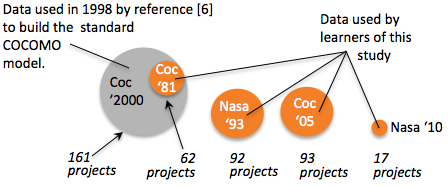
\includegraphics[width=3.2in]{datasets1.png}
\end{center}
\caption{\ADD{Projects in this study (COC81 is a subset of COC'2000).}}\label{fig:dataused}
\end{figure}



\begin{figure}[!b]

~\\~\\

\begin{center}
{\scriptsize
\begin{tabular}{r|@{~}r|@{~}r|@{~}r|@{~}l}

Types of projects& COC81 & NASA93& COC05 &NASA10\\\hline 
Avionics&     &26&10&17\\\hline
Banking&       &      &13&     \\\hline
Business apps/data processing&7&4&31&  \\\hline   
Control&9&18&13&     \\\hline
Human-machine interaction&12&       &       &     \\\hline
Military, ground&       &       &8&     \\\hline
Misc&5&4&5&     \\\hline
Mission Planning&      &16&       &     \\\hline
SCI scientific application&16&21&11&     \\\hline
Support (tools, utilities, etc)&7&        &       &   \\\hline  
Sys (OS, compilers, sensors,etc)&7&3&2&     
     

%% NASA10& COC05 & NASA93& COC81 & Types of projects\\\hline\hline
%%      &     5 &4      &       & Misc\\\hline
%%      &       &        &  7   &  Support (tools, utilities, etc)\\\hline
%%      &      8&       &       & Military, ground\\\hline
%%      &      13&      &       & Banking\\\hline
%%      &      2&3      & 7     & Sys (OS, compilers, sensors,etc)\\\hline
%%      &      31&4     &  7    & Business apps/data processing\\\hline
%%      &       &16      &      & Mission Planning\\\hline
%%      &     13  &18     &   9 & Control\\\hline
%%      &       &       & 12    & Human=machine interaction\\\hline
%%      &      11& 21     & 16   & SCI scientific application\\\hline
%%  17  &     10 &26      &     & Avionics Monitoring
\end{tabular}}

~\\~\\

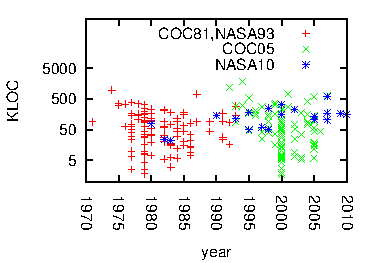
\includegraphics[width=2.3in]{yearLOC.pdf}
\noindent
\end{center}
\caption{Projects used by the learners in this study. \fig{cparems}
shows project attributes. 
COC81 is the original data from 1981 COCOMO book~\cite{boehm81}. 
This comes from projects dating 1970 to 1980.
NASA93 is NASA data collected  in the early 1990s
 about software that supported  the planning activities for the International
Space Station. 
Our two other data sets are COC05 and NASA10 (these data sets
are proprietary and 
cannot be released to the research community). 
The non-proprietary data  (COC81 and NASA93) is available at
http://openscience.us/repo.
}\label{fig:types}
\end{figure}

Using that data,  the experiments of this paper conclude that
the answer to all  our  research questions is
``no''.  
The RQ1 experiments show that good estimates use many variables
and  poorer estimates result from   some trite calculation based on KLOC.   
Hence,  we can make some degree of
error in our KLOC estimates without damaging the overall estimation process (see RQ5).

As to the other research questions (R2,R3,R4), those results mean that 
the continued
use of parametric estimation can still be endorsed.
What COCOMO, or other parametric
estimation models, can offer largely contains the
fundamentals for making estimation decisions
from expert-Delphi, as well as well calibrated
tuning factors from over 40 years of
industrial data.  We would advise
researchers {\em not} to ignore these fundamentals.
%% These new model  are of many types.
%% Older approaches
%% used a fixed set of parameters (e.g
%%  COCOMO, FPA~\cite{albrecht79},
%% SLIM~\cite{putnam80}).
%% More recent work has applied methods
%% that can accept a wider range  parameters including
%% analogy-based methods~\cite{shepperd97} and 
%% combination methods that take advantage of
%% multiple simpler methods. For example, Corazza
%% et al.~\cite{cora10} uses tabu search to configure support vector
%% machines for effort estimation.
%% Other approaches  combine
%% hundreds of different methods-- see
%%  Menzies et al.~\cite{me06d} or 
%% Kocaguneli~\cite{me11a}.
%% Yet other approaches use
%% temporal learning methods  incrementally modify past
%% models or data to make estimates on new projects (see the 
%% pioneering work of Lokan and Mendes~\cite{lokan06}, or more recent
%% work by Minku and Yao~\cite{minku14})).
%% XXX implications for more researh
%% {\scriptsize
%% \Tree [.Projects\ can\\have\ COCOMO\\attributes? 
%%            [.yes [.Dozens\ of\\examples? 
%%                      [.yes COCOMO ]
%%                      [.no  COCOMO-II\\+\ COCOUUT\\+\ Column\ prune ] ] ] 
%%            [.no  [.Dozens\ of\\examples? 
%%                       [.yes Try\ parametric\\methods\ first ]
%%                       [.no  Case-based\\reasoning ] ] ] ]
%% }

More generally, these results make us question 
some of the newer (and supposedly better) innovative techniques for effort estimation.  
The unique and highly variable characteristics of SE
project data place great limitation on the results
obtained by naively applying some brand-new
algorithm.  Perhaps the best future direction is to
investigate how innovative new techniques can extend
(rather than replace) existing and successful
estimation methods.  Some experiments in this paper
are a starting point for that investigation.


\section{Background}





\subsection{Parameter- vs Model- vs Delpi-based Estimation}

\begin{changed}

COCOMO is a parametric method; i.e. it is a 
{\em model-based} method that (a)~assumes that the target model has a particular structure,
then (b)~uses model-based methods to fill in the details of that structure (e.g. to set some tuning parameters).


One of the myths of effort estimation is that no one used model-based estimation and that
estimates are always better done using expert-based guess-timation, a.k.a. {\em Delphi-based} methods\footnote{The mythological oracle of Delphi spoke for the god Apollo to answered questions  about colonization, religion, and power.}.
As seen in the introduction, model-based
parametric methods are  widely used in industry and
are strongly advocated by professional socients.
Also, 
while it is true that Delphi-based estimation is a common practice~\cite{boehm00a}, this is not to say that this should be recommended as the {\em best} or {\em only} way to make estimates:
\bi 
\item
Jorgensen~\cite{Jorgensen2004} reviews studies 
comparing  model- and Delphi- based estimation and concludes that there
there is no clear case that delph-methods are better.
\item 
Valerdi~\cite{valerdi11} lists the
cognitive biases that can make an expert offer poor Delphi-estimates.
\item Passos et al. show that many
commercial software engineers generalize from their
first few projects to all future
projects~\cite{passos11}.
\item
Jorgensen \& Gruschke~\cite{jorgensen09} document how
  commercial  ``gurus'' rarely use lessons
  from past projects to improve their future Delphi-estimates. 
 They offer examples where this
  failure to revise prior beliefs   leads to poor
 Delphi-based estimates.
  \ei 
Much research has concluded that best    estimations come from {\em combining} the predictions
from {\em multiple oracles}~\cite{koc11a,chulani99,baker07,valerdi11}.  
 \begin{figure}[!b]
{\scriptsize
\begin{center}
\begin{tabular}{|p{0.2in}|p{1.46in}|p{0.77in}|p{0.77in}|p{0.77in}|}\hline

 & Definition & Low-end = \{1,2\}
 &Medium =\{3,4\} &High-end= \{5,6\} \\\hline


\multicolumn{5}{l}{Scale factors:}\\\hline
Flex   &  development flexibility   & development process
rigorously defined & some guidelines, which can be relaxed & only
general goals defined\\\hline

Pmat    & process maturity  &  CMM level 1 &   CMM level 3  &  CMM level 5 \\\hline

Prec & precedentedness  &  we have never built this kind
of software before &    somewhat new &
thoroughly familiar \\\hline

Resl &  architecture or risk resolution  &  few interfaces
defined or few risks eliminated  &  most interfaces defined or most
risks eliminated   & all interfaces defined or all risks
eliminated\\\hline

Team  &   team cohesion  &  very difficult interactions &
basically co-operative  &  seamless interactions\\\hline


\multicolumn{5}{l}{Effort multipliers}\\\hline
acap  &  analyst capability  &  worst 35\% &   35\% - 90\% &  best 10\% \\\hline

aexp   &  applications experience  &  2 months &   1 year  &  6 years\\\hline

cplx   &  product complexity   & e.g. simple read/write
statements & e.g. use of simple interface widgets  &  e.g.
performance-critical embedded systems\\\hline

data   &  database size 
(DB bytes/SLOC) &
10 & 100 &    1000 \\\hline

docu   &  documentation   & many life-cycle phases not
documented      & &  extensive reporting for each life-cycle phase\\\hline

ltex   &  language and tool-set experience   & 2 months  &  1
year & 6 years \\\hline

pcap   &  programmer capability  &  worst 15\%   & 55\%  &  best 10\% \\\hline


pcon   &  personnel continuity \newline
(\% turnover per year) &
    48\% &    12\%  & 3\% \\\hline

plex   &  platform experience  &  2 months  &  1 year  &  6 years\\\hline


pvol   &  platform volatility ($\frac{frequency~of~major~changes}{frequency~of~minor~changes}$) &
$\frac{12~months}{1~month}$   & $\frac{6~months}{2~weeks}$ &
$\frac{2~weeks}{2~days}$\\\hline



rely   &  required
reliability &   errors are slight inconvenience  &  errors are easily
recoverable   & errors can risk human life\\\hline




ruse   &  required
reuse &   none &    multiple program  & multiple product lines\\\hline

sced  &   dictated development\newline schedule &    deadlines moved to
75\% of the original estimate &  no change
&  deadlines moved back to  160\% of original estimate\\\hline

site   &  multi-site development   & some contact: phone, mail&
some email  &  interactive multi-media\\\hline

stor  &   required \% of available
RAM & N/A
 &   50\% &  95\% \\\hline


time  &   required \% of available CPU &
N/A&     50\%
   &  95\% \\\hline


tool   &  use of software tools  &  edit,code,debug &&
integrated with life cycle\\\hline
\end{tabular}
\end{center}
} \caption{COCOMO-II attributes.}
\label{fig:cparems}
\end{figure}
Note that it is far easy faster to apply this double-check strategy using Delphi+model-based methods 
than by comparing the estimates from multiple Delphi teams.
For example, all the model-based methods  studied in this paper can generate estimates
in just a few seconds. In comparison, Delphi-based estimation is orders of magnitude slower-- as seen in  
Valerdi's  
COSYSMO Delphi-method.
While a strong proponent of this approach, Valerdi concedes that 
``(it is)  extremely time
consuming when large sample sizes are needed''~\cite{valerdi11}.
For example, he once
recruited 40 experts to three Delphi sessions, each of which ran for three hours.
Assuming a 7.5 hour day,
then that study took \[3*3*40 /7.5 = 48\; \mathit{days}\]

COSYSMO is an elaborate Delphi-based method. An alternate, more lightweight Delphi-method is  ``planning poker''~\cite{molokk08} where
participants offer anonymous
``bids'' on the 
completion time for a project. If  the bids are widely divergent, then the factors
leading to that disagreement elaborated and debated. This cyclic of bid+discuss continues
until a consensus has been reached.

While planning poker is widely advocated in the agile community,
there are surprisingly few studies assessing this method (one rare exception is~\cite{molokk08}).
Further,   planning poker is used to assessing effort
for particular tasks in the scrum backlog-- which is a different and simpler task
than the {\em initial} estimation of  large-scale
projects. This is an important issue since, for larger
projects, that initial budget allocation may require a significant amount of intra-organizational lobbying between groups with competing concerns. For such large-estimate-projects, if can
be challenging to change the initial budget allocation. Hence, it is important to get
that initial estimate as accurate as possible.

\end{changed}
\subsection{COCOMO: Origins and Development}
These concerns with  Delphi  date
back many decades and were the genesis for  COCOMO. In 1976, Robert Walquist (a TRW division general manager)
told  Boehm: \begin{quote}{\em ``Over the last three
weeks, I've had to sign proposals that committed us
to budgets of over \$50 million to develop the
software.  In each case, nobody had a good
explanation for why the cost was \$50M vs. \$30M or
\$100M, but the estimates were the consensus of the
best available experts on the proposal team.  We
need to do better. Feel free to call on experts
\& projects with data on previous software cost.''}\end{quote}



TRW had a previous model that worked well for a part
of TRW's software business~\cite{wol74}, but it
did not relate well to the full range of embedded
software, command and control software, and
engineering and scientific software involved in
TRW's business base.  Having access to experts and
data was a rare opportunity, and a team involving
Ray Wolverton, Kurt Fischer, and Boehm conducted a
series of meetings and Delphi exercises to find
the relative significance of various  cost
drivers. Combining local expertise  and data, plus some prior results 
such as~\cite{putnam76,black77,herd77,watson77},  and early versions of the RCA
PRICE S model~\cite{frei79}, a model called SCEP was created (Software Cost
Estimation Program).
Except for
one explainable outlier, the estimates for
 20 projects with solid data were within 30\% of
the actuals, with most within 15\% of the actuals.

\begin{figure}[!t]
\begin{lstlisting}
_  = None;  Coc2tunings = [[
#              vlow  low   nom   high  vhigh  xhigh   
# scale factors:
'Flex',        5.07, 4.05, 3.04, 2.03, 1.01,     _],[
'Pmat',        7.80, 6.24, 4.68, 3.12, 1.56,     _],[
'Prec',        6.20, 4.96, 3.72, 2.48, 1.24,     _],[
'Resl',        7.07, 5.65, 4.24, 2.83, 1.41,     _],[
'Team',        5.48, 4.38, 3.29, 2.19, 1.01,     _],[
# effort multipliers:        
'acap',        1.42, 1.19, 1.00, 0.85, 0.71,    _],[
'aexp',        1.22, 1.10, 1.00, 0.88, 0.81,    _],[
'cplx',        0.73, 0.87, 1.00, 1.17, 1.34, 1.74],[
'data',           _, 0.90, 1.00, 1.14, 1.28,    _],[
'docu',        0.81, 0.91, 1.00, 1.11, 1.23,    _],[
'ltex',        1.20, 1.09, 1.00, 0.91, 0.84,    _],[
'pcap',        1.34, 1.15, 1.00, 0.88, 0.76,    _],[ 
'pcon',        1.29, 1.12, 1.00, 0.90, 0.81,    _],[
'plex',        1.19, 1.09, 1.00, 0.91, 0.85,    _],[ 
'pvol',           _, 0.87, 1.00, 1.15, 1.30,    _],[
'rely',        0.82, 0.92, 1.00, 1.10, 1.26,    _],[
'ruse',           _, 0.95, 1.00, 1.07, 1.15, 1.24],[
'sced',        1.43, 1.14, 1.00, 1.00, 1.00,    _],[ 
'site',        1.22, 1.09, 1.00, 0.93, 0.86, 0.80],[ 
'stor',           _,    _, 1.00, 1.05, 1.17, 1.46],[
'time',           _,    _, 1.00, 1.11, 1.29, 1.63],[
'tool',        1.17, 1.09, 1.00, 0.90, 0.78,    _]]

def COCOMO2(project,  a = 2.94, b = 0.91, # defaults
                      tunes= Coc2tunings):# defaults 
  sfs ems, kloc  = 0,1,22          
  scaleFactors, effortMultipliers = 5, 17
  for i in range(scaleFactors):
    sfs += tunes[i][project[i]]
  for i in range(effortMultipliers):
    j = i + scaleFactors
    ems *= tunes[j][project[j]] 
  return a * ems * project[kloc] ** (b + 0.01*sfs) 
\end{lstlisting}
\caption{COCOMO-II: effort estimates from a {\em project}.
Here, {\em project} has up to 24 attributes  (5 scale
factors plus 17 effort multipliers plus KLOC plus. in the training data, the actual effort).
Each attribute except KLOC and effort is scored
using the scale very low = 1, low=2, etc.
For an explanation of the attributes shown in
green, see \fig{cparems}.}\label{fig:coc2}
\end{figure}

%%  and worked with projects to gather uniform
%% software cost driver and effort data on its 1970s
%% large software projects.  The data definitions were
%% based on TRW’s waterfall-model based software
%% development policies and standards. They also
%% benefited from a concurrent surge in publications
%% describing software cost estimation models such as~\cite{putnam76,black77,herd77,watson77} and early versions of the RCA
%% PRICE S model~\cite{frei79}.
%% SCEP  became standard practice for
%% large TRW projects; and a TRW Office of Software
%% Cost Estimation was established to provide its usage
%% support, training, data collection and analysis, and
%% evolution, which continues to this day.


%% The conclusion for that work
%% was that a reasonably accurate model could
%% be developed, but that proposals and projects should
%% complement its results with expert-judgment based
%% estimates, and reconcile their results where
%% necessary.  
%% It was given the name SCEP, for Software Cost
%% Estimation Program; its use along with expert
%% judgment estimates became standard practice for
%% large TRW projects; and a TRW Office of Software
%% Cost Estimation was established to provide its usage
%% support, training, data collection and analysis, and
%% evolution, which continues to this day.

%% SCEP was highly successful in proposal and
%% management use, but it was proprietary to TRW and
%% could not be used by customers to evaluate other
%% companies' cost estimates.  Thus, TRW became
%% receptive to having a version that generalized
%% beyond TRW experience but was still accurate for
%% TRW.  

After  gathering some further data from subsequent
TRW projects and about 35 projects from teaching
software engineering courses at UCLA and USC along
with commercial short courses on software cost
estimation, Boehm was able to gather 63 data points
that could be published and to extend the model to
include alternative development modes that covered
other types of software such as business data
processing.  The resulting model was called the
COnstructive COst MOdel, or COCOMO, and was
published along with the data in the book Software
Engineering Economics~\cite{boehm81}. 
In COCOMO-I, project attributes
were scored using just a few coarse-grained values (very low,
low, nominal, high, very high). These attributes
are {\em effort multipliers} where
a off-nominal value changes the estimate by some number
greater or smaller than one.
In COCOMO-I, all attributes (except KLOC)
influence effort in a linear manner.

Following the release of COCOMO-I Boehm created a consortium for
industrial organizations using COCOMO .
The consortium
collected information on 161 projects from commercial,
aerospace, government, and non-profit organizations.
Based on an analysis of those 161 projects, Boehm
 added  new attributes called {\em scale factors}
that had an {\em exponential impact}
on effort (e.g. one such attribute was process maturity).
Using that new data, Boehm and his colleagues developed
the  {\em tunings} shown in \fig{coc2} that
map the project descriptors (very low, low, etc)
into the specific values used in the COCOMO-II model
(released in 2000~\cite{boehm00b}):
\begin{equation}\label{eq:cocII}
\mathit{effort}=a\prod_i EM_i *\mathit{KLOC}^{b+0.01\sum_j SF_j}
\end{equation}
Here, {\em EM,SF} are  effort multipliers and scale
factors and
 $a,b$ are the {\em local calibration} parameters (with default values of 2.94 and 0.91).
Also, {\em effort}
measures ``development months'' where one month
is 152 hours of work  (and includes development and management hours).
For example, if {\em effort}=100, then according to COCOMO,
five developers would finish
the project in 20 months.



Note that, from \eq{cocII},
the minimum  
effort  is bounded by the  {\em sum} of the minimum scale factors
and the {\em product} of the minimum effort multipliers.
Similar expressions hold for the  maximum effort estimate. Hence,
for a given KLOC, the range of values is given by:
\[
0.18*\mathit{KLOC}^{0.97}  \le \mathit{effort} \le 154*\mathit{KLOC}^{1.23}\]
Dividing the minimum and maximum values results in an  expression showing
how    effort can vary for any given KLOC.: 
\begin{equation}\label{eq:ration}
154/0.18 *\mathit{KLOC}^{1.23 - 0.97} = 856*\mathit{KLOC}^{0.25}
\end{equation}
 



 
\subsection{COCOMO and Local Calibration}\label{sect:coconut}
When local data is scarce, approximations can be used to
tune a model using just a handful of examples.  
 COCOMO   {\em local calibration} pocedure, adjusts the impact of the scale factors and effort
multipliers by tuning the  $a,b$ values of Equation~\ref{eq:cocII}
while keeping constant the other values of the tuning matrix
shown in \fig{coc2}. Effectively, local calibration trims
a 23 variable model
into a model with two variable: (one  to adjust the linear effort
multipliers, and another to adjust the exponential scale factors).

Menzies' preferred local calibration procedure is the COCONUT
procedure of \fig{coconut} (first written in 2002
and first published in 2005~\cite{me04h}). 
For some number of {\em repeats},
COCONUT will {\em ASSESS} some {\em GUESSES} 
 for $(a,b)$ by applying them to some
{\em training} data. If any of these guesses prove to
be {\em useful} (i.e. reduce the estimation error) then COCONUT will recurse after
{\em constricting} the guess range for $(a,b)$ by some amount (say, by $2/3$rds). COCONUT terminates
when (a)~nothing better is found at the current level of recursion
or (b)~after 10 recursive calls-- at which point the guess range
has been constricted to  $(2/3)^{10}\approx 1$\% of the initial range.


\begin{figure}[!t]
\begin{lstlisting}
def COCONUT(training,          # list of projects
            a=10, b=1,         # initial  (a,b) guess
            deltaA    = 10,    # range of "a" guesses 
            deltaB    = 0.5,   # range of "b" guesses
            depth     = 10     # max recursive calls
            constricting=0.66):# next time,guess less
  if depth > 0:
    useful,a1,b1= GUESSES(training,a,b,deltaA,deltaB)
    if useful: # only continue if something useful
      return COCONUT(training, 
                     a1, b1,  # our new next guess
                     deltaA * constricting,
                     deltaB * constricting,
                     depth - 1)
  return a,b

def GUESSES(training, a,b, deltaA, deltaB,
           repeats=20): # number of guesses
  useful, a1,b1,least,n = False, a,b, 10**32, 0
  while n < repeats:
    n += 1
    aGuess = a1 - deltaA + 2 * deltaA * rand()
    bGuess = b1 - deltaB + 2 * deltaB * rand()
    error  = ASSESS(training, aGuess, bGuess)
    if error < least: # found a new best guess
      useful,a1,b1,least = True,aGuess,bGuess,error
  return useful,a1,b1

def ASSESS(training, aGuess, bGuess):
   error = 0.0
   for project in training: # find error on training
     predicted = COCOMO2(project, aGuess, bGuess)
     actual    = effort(project)
     error    += abs(predicted - actual) / actual
   return error / len(training) # mean training error
\end{lstlisting}
\caption{COCONUT  tunes  $a,b$ 
of \fig{coc2}'s COCOMO function.}\label{fig:coconut}
\end{figure}

 


%Local calibration
%can dramatically improve the effort estimates
%from COCOMO. For example, in one result shown below, 
%COCONUT reduced the variance in the
%estimates  by a factor of seven
%(from 214\% to 34\%).




\section{Experimental Methods} 
%% \begin{figure*}
%% {\scriptsize
%% \begin{verbatim}
%% vl=1; l=2; n=3; h=4; vh=5; xh=6

%% def nasa93():  
%%   return dict( 
%%     names= [ 
%%      'Prec','Flex','Resl','Team','Pmat',  # scale factors
%%      'rely','data','cplx','ruse','docu',  # effort multipliers
%%      'time','stor','pvol','acap','pcap',  # effort multipliers
%%      'pcon','aexp','plex','ltex','tool',  # effort multipliers
%%      'site', 'sced',                      # effort multipliers
%%      'kloc','effort],

%%     projects=[                                      
%%      #Scale        
%%      #factors    Effort multipliers                Kloc   Effort
%%      #---------- --------------------------------- -----  ------
%%      [h,h,h,vh,h,h,l,h,n,n,n,n,l,n,n,n,n,n,h,n,n,l, 25.9, 117.6],
%%      [h,h,h,vh,h,h,l,h,n,n,n,n,l,n,n,n,n,n,h,n,n,l, 24.6, 117.6],
%%      [h,h,h,vh,h,h,l,h,n,n,n,n,l,n,n,n,n,n,h,n,n,l,  7.7,  31.2],
%%      [h,h,h,vh,h,h,l,h,n,n,n,n,l,n,n,n,n,n,h,n,n,l,  8.2,  36  ],
%%      # ... 
%%     ])
%% \end{verbatim}}
%% \caption{Sample data used in this project (first four rows of NASA93).}\label{fig:data1}
%% \end{figure*}





\begin{figure}[!t]
\begin{lstlisting}
def RIG():
 DATA = { COC81, NASA83, COC05, NASA10 }
 for data in DATA # e.g. data = COC81
     mres= {}
     for learner in LEARNERS # e.g. learner = COCONUT
       n = 0
       10 times repeat: 
         for project in DATA #  e.g.  one project
           training = data - project # leave-one-out
           model    = learn(training)
           estimate = guess(model, project)
           actual   = effort(project)
           mre      = abs(actual - estimate)/actual
           mres[learner][n++] = mre
     print rank(mres) # some statistical tests
\end{lstlisting}
\caption{The experimental rig used in this paper.}\label{fig:rig}
\end{figure}



\subsection{Choice of Experimental Rig}




``Ecological inference''
is the conceit 
that what holds for all, also holds for parts 
of the population~\cite{posnet11,me12d}.
To avoid ecological inference,
our  rig in Figure~\ref{fig:rig}
runs separately for each data set.  


Since some of our methods include a stochastic
algorithm (the COCONUT algorithm of \fig{coconut}),
we repeat our experimental rig   $N=10$ times
(10 was selected since, after experimentation, we
found our results looked the same at $N=8$ and
$N=16$).



\begin{changed}
It is important to note that Figure~\ref{fig:rig} is a ``leave-one-out experiment''; i.e.
training is conducted on all-but-one example, then tested
on an ``holdout'' example not seen in training. This separation of training and testing
data is of particular
importance in this study. 
As shown in \fig{types}, our  data sets (NASA10, COC81, NASA93, and COC05)
contain information on 17, 63, 92, and 93  projects, respectively. When fitted to
the   24 parameters of the standard COCOMO model  (shown in \fig{cparems}),
there may not be enough information to constrain the learning-- which means that it is theoretically
possible that data could be fitted to almost anything (including {\em spurious noise}).
To detect such spurious models, it is vital to test the learned model against some
outside source such as the holdout example.
\end{changed} 

We assess  
performance via the magnitude of the relative error; i.e. 
\mbox{$ \mathit{MRE}=\frac{abs(\mathit{actual} - \mathit{predicted})}{\mathit{actual}}$}. 
Shepperd \& MacConnell~\cite{shepperd12a} propose
another measure that reports the performance as a
ratio of some other, much
simpler, ``straw man'' approach (they recommend the
mean effort value of $N>100$ random samples of the
training data). At first, we used the Shepperd \&
MacConnell approach for this work but found that
their straw man had orders of magnitude larger error
than all the results shown here. Hence, we adopt the
spirit, but not the letter, of their proposal and
compare all our results against the LOC(n) ``straw
man'' method discussed below.
 

\subsection{Choice of Learners}\label{sect:whatlearn}

Our LOC(n) ``straw man'' 
estimators just uses  lines of code
in the $n$ nearest projects. For distance,
we use:
\begin{equation}\label{eq:dist}
\mathit{dist}(x,y) = \sqrt{\sum_i w_i (x_i-y_i)^2}
\end{equation} 
where $x_i,y_i$ 
are values normalized 0..1 for the range min..max
and $w_i$ is a weighting factor (defaults to $w_i=1$).
When  estimating from $n>1$ neighbors,
we combines estimates via the triangle 
function of  Walkerden
and Jeffery~\cite{Walkerden1999}; 
e.g.. for $loc(3)$, the  estimate
from the first, second, third closest neighbor with estimates
$a,b,c$ is 
\begin{equation}\label{eq:tri}
\mathit{effort} = (50a + 33b + 17c)/100
\end{equation}
Apart from the LOC ``straw man'',
we also compare COCOMO-II and COCONUT with CART,
Knear(n), TEAK, and PEEKING2. 
These  methods were  selected, for the following reasons.
TEAK  and PEEKING2   represent   recent innovations in effort
estimation~\cite{koc11b,papa13}.  
CART and Knear(n) are more traditional methods  that proved their value  in the 1990s~\cite{shepperd97,Walkerden1999}. That said, CART and Knear(n)
still have currency: 
recent results from IEEE TSE 2008 and 2012 still endorse their  use for effort estimation~\cite{dejaeger12,koc11a,keung2008b}).
Also, according to the Shaw's timetable for industry adoption of research innovations
(discussed in the introduction),  CART and Knear(n) should now be mature enough for industrial use.


CART~\cite{breiman84} is an {\em iterative dichotomization} algorithm
that finds the attribute that most divides the data such that
the variance of the goal variable in each division is minimized.
The algorithm then recurses on each division. 
Finally, the cost data in the leaf divisions
is averaged to generate the estimate. 


Knear(n) estimates a new project's effort
by a nearest neighbor  method~\cite{shepperd97}. Unlike LOC(n),
a Knear(n) method uses all attributes
(all scale factors and effort multipliers as well as lines of code)
to find the {\em n-th} nearest projects in the training data. 
Knear(3) combines efforts from three nearest neighbors using
Equation~\ref{eq:tri}.
Knear(n) is an example of CBR; i.e.  {\em case-based reasoning}.
CBR for effort estimation was 
first pioneered by Shepperd \& Schofield
in 1997~\cite{shepperd97}.
  Since then, it 
has been used extensively in software effort
estimation~\cite{Auer2006,Walkerden1999,%
  Kirsopp2002,shepperd97,kadoda00,Li2008,Li2006,Li2007,Li2009a,
  keung2008a,keung2008b,keung2008c}.  
There are several reasons  for this. Firstly, 
it works even if the domain data is sparse~\cite{Myrtveit}.
Secondly, 
unlike other predictors, it makes no assumptions about data
distributions or some  underlying parametric model. 

\begin{changed}
TEAK is built
on the assumption that spurious noise leads to large variance in the recorded efforts~\cite{koc11b}.
TEAK's pre-processor removes such regions of high variance as follows.
First, it  applies greedy agglomerate clustering  to generate a tree of clusters.
Next, it reflects on the variance
of the efforts seen in each sub-tree and discards the sub-trees with largest variance. Estimation is then performed
on the surviving examples.

PEEKING2~\cite{papa13} is a far more aggressive ``data pruner'' than TEAK and combines   data reduction operators, 
feature weighting,  and PCA. PEEKING2 is described in  \fig{peeking}.
\end{changed}


\begin{figure}[!t]
\small
\begin{tabular}{|p{.95\linewidth}|}\hline
\bi
\item
PEEKING2's feature weighting scheme changes  $w_i$ in \eq{dist}  according to how much an attribute
can divide and reduce the variance of the effort data (the {\em greater} the reduction, the
{\em larger} the $w_i$ score).  
\item
PEEKING2's PCA tool used an accelerated   principle component analysis that synthesises  new
attributes $e_i, e_2,...$
that extends across the dimension of greatest  variance in the data  with attributes $d$.  
PCA  combines
redundant  variables into a smaller set of variables  (so $e \ll d$) since those
redundancies become (approximately) parallel lines
in $e$ space. For all such redundancies \mbox{$i,j \in d$}, we 
can ignore $j$ 
since effects that change over $j$ also
change in the same way over $i$.
PCA is also useful for skipping over noisy variables from $d$-- these
variables are effectively ignored since    they  do not contribute to the variance in the data.
\item
PEEKING2's prototype generator  clusters the data along the dimensions
found by accelerated PCA. Each cluster is then replaced with a ``prototype'' generated from
the median value of all attributes in that cluster. Prototype generation is a useful tool for
handling outliers: large groups of outliers get their own cluster; small sets of outliers
get ignored via median prototype generation.
\item
PEEKING2 generates estimates for a test case by finding its nearest cluster,
then the two nearest neighbors within that cluster  (where ``near''
is computed using \eq{dist} plus feature weighting). If these neighbors are found at distance
$n_1,n_2, n_1 < n_2$ and have effort values $E_1,E_2$ then the final estimate is an extrapolation
favoring the closest one:
\ei
\[
n=n_i+n_2;\;\mathit{estimate}=E_1\frac{n_2}{n} + E_2\frac{n_1}{n}
\]\\\hline
\end{tabular} 
\caption{Inside PEEKING2~\cite{papa13}.}\label{fig:peeking}
\end{figure}




%% Finally, one more learner is explored, just to handle
%% a possible criticism of this work. This paper
%% reports that a COCOMO method works best on four data sets
%% that were all collected using the COCOMO ontology.
%% ``Of course COCOMO does best,'' says this particular
%% criticism, ``since all the test cases are already
%% written in COCOMO''.  To test this, we need a rather
%% particular experimental method: (1)~a data set where
%% projects are expressed
%% in {\em both} the COCOMO attributes of \fig{cparems}
%% as well as other attributes; and (2)~our best COCOMO
%% learner applied to our best


%XX threats to validity

%% Our final experiment 
%% check if the results of this paper are just due
%% to COCOMO-based learners being applied to COCOMO data
%% (see \tion{other}). Hence, we 
%% needed one more learner that was more representative
%% of recent work than CART or Knear(n). 
%% Such a learner is the 
%% PEEKING algorithm of Papakroni~\cite{papa13}.
%% PEEKING
%% is a non-parametric response surface method that generates estimates for a project by
%%  interpolating between
%% the two nearest centroids found by a clustering algorithm.
%%  This interpolation is weighted by the
%% distance to each centroid (and the estimate from
%% the closer centroid has more weight, see \fig{PEEKING}).
%% That is,  PEEKING is any example of a {\em prototype learner}~\cite{chang74}
%%  that replaces $N$ examples with $M \ll N$ most informative ``prototypes'' (in this case,
%% the cluster centroids).
%% Prototype learners mitigate for data outliers since 
%% noisy outliers disappear from the prototypes~\cite{chang74}.
%% In an extensive study,
%% Papakroni~\cite{papa13} found that PEEKING's predictions where (1)~ competitive
%% with random forests and  Naive Bayes (for defect prediction)
%% and (2)~regression trees and linear regression (for effort estimation).




%% \begin{figure}[!t]
%% \begin{lstlisting}
%% def PEEKING(data,project):
%%    prototypes= WHERE(data)
%%    neighbors = distances(project,prototypes) 
%%    one, two  = neighbors[0],neighbors[1] #two closest
%%    d1, d2    = dist(one,project), dist(two,project)
%%    w1, w2    = 1 /d1,  1 /d2 #closest has most weight
%%    est1, est2= effort(one), effort(two)
%%    return (w1*est1 + w2*est2) / (w1 + w2) 
%% \end{lstlisting}
%% \caption{PEEKING: a non-parametric response surface method that 
%% generates estimates from a  set of piecewise linear approximations.
%% PEEKING builds its clusters using the WHERE spectral clusterer~\cite{me11m}
%% that
%% recursively divides projects
%% synthesized by a 
%% principle component analysis to filters out irrelevant attributes. For reasons of efficiency, WHERE
%%   uses the $O(2N)$ FASTMAP
%%   method~\cite{platt05,Faloutsos1995} rather than
%%   the standard $O(N^2)$ method to find these
%%   principle components~\cite{Du2008}.
%% }\label{fig:PEEKING}
%% \end{figure}


\subsection{Choice of Statistical Ranking Methods}\label{sect:stats}
The last line of our experimental rig shown in
\fig{rig} {\em rank}s multiple methods for learning
effort estimators.
This study ranks methods using the Scott-Knott
procedure recommended by Mittas \& Angelis in their 2013
IEEE TSE paper~\cite{mittas13}.  This method
sorts a list of $l$ treatments with $ls$ measurements by their median
score. It then
splits $l$ into sub-lists $m,n$ in order to maximize the expected value of
 differences  in the observed performances
before and after divisions. E.g. for lists $l,m,n$ of size $ls,ms,ns$ where $l=m\cup n$:
 \[E(\Delta)=\frac{ms}{ls}abs(m.\mu - l.\mu)^2 + \frac{ns}{ls}abs(n.\mu - l.\mu)^2\]
Scott-Knott then applies some statistical hypothesis test $H$ to check
if $m,n$ are significantly different. If so, Scott-Knott then recurses on each division.
For example, consider the following data collected under different treatments {\em rx}:

{\scriptsize \begin{verbatim}
        rx1 = [0.34, 0.49, 0.51, 0.6]
        rx2 = [0.6,  0.7,  0.8,  0.9]
        rx3 = [0.15, 0.25, 0.4,  0.35]
        rx4=  [0.6,  0.7,  0.8,  0.9]
        rx5=  [0.1,  0.2,  0.3,  0.4]
\end{verbatim}}
\noindent
After sorting and division, Scott-Knott declares:
\bi
\item Ranked \#1 is rx5 with median= 0.25
\item Ranked \#1 is rx3 with median= 0.3
\item Ranked \#2 is rx1 with median= 0.5
\item Ranked \#3 is rx2 with median= 0.75
\item Ranked \#3 is rx4 with median= 0.75
\ei
Note that Scott-Knott found  little
difference between rx5 and rx3. Hence,
they have the same rank, even though their medians differ.

Scott-Knott is better than an 
 all-pairs hypothesis test of all methods; e.g. six treatments
can be compared \mbox{$(6^2-6)/2=15$} ways. 
A 95\% confidence test run for each comparison has  a very low total confidence: 
\mbox{$0.95^{15} = 46$}\%.
To avoid an all-pairs comparison, Scott-Knott only calls on hypothesis
tests {\em after} it has found splits that maximize the performance differences.
 
For this study, our hypothesis test $H$ was a
conjunction of the A12 effect size test of  and
non-parametric bootstrap sampling; i.e. our
Scott-Knott divided the data if {\em both}
bootstrapping and an effect size test agreed that
the division was statistically significant (99\%
confidence) and not a ``small'' effect ($A12 \ge
0.6$).

For a justification of the use of non-parametric
bootstrapping, see Efron \&
Tibshirani~\cite[p220-223]{efron93}.
For a justification of the use of effect size tests
see Shepperd\&MacDonell~\cite{shepperd12a}; Kampenes~\cite{kampenes07}; and
Kocaguenli et al.~\cite{kocharm13}. These researchers
warn that even if an
hypothesis test declares two populations to be
``significantly'' different, then that result is
misleading if the ``effect size'' is very small.
Hence, to assess 
the performance differences 
we first must rule out small effects.
Vargha and Delaney's
non-parametric 
A12 effect size test 
explores
two lists $M$ and $N$ of size $m$ and $n$:
\[A12 = \left(\sum_{x\in M, y \in N} 
\begin{cases} 
1   & \mathit{if}\; x > y\\
0.5 & \mathit{if}\; x == y
\end{cases}\right) / (mn)
\]
This expression computes the probability that numbers in one sample are bigger than in another.
This test was recently 
endorsed by Arcuri and Briand
at ICSE'11~\cite{arcuri11}.





\begin{figure}[!t]
 
{\scriptsize
{\bf NASA10 (new NASA data up to 2010):}

{\scriptsize \begin{tabular}{l@{~~~}l@{~~~}r@{~~~}r@{~~~}c}
\arrayrulecolor{darkgray}
\rowcolor[gray]{.9}  rank & treatment & median & IQR & 
%min= 20, max= 117
\\
  1 &      COCOMO-II &    42  &  35 & \quart{4}{36}{22}{82} \\
\hline  2 &      COCONUT &    47  &  34 & \quart{19}{35}{27}{82} \\
\hline  3 &       loc(3) &    49  &  97 & \quart{0}{99}{29}{82} \\
  3 &       loc(1) &    67  &  44 & \quart{12}{45}{48}{82} \\
\end{tabular}}

% :learn 4.64 :analyze 1.69 :boots 3 effects 5 :conf 0.970299

~\\

{\bf COC05 (new COCOMO data up to 2005):}

{\scriptsize \begin{tabular}{l@{~~~}l@{~~~}r@{~~~}r@{~~~}c}
\arrayrulecolor{darkgray}
\rowcolor[gray]{.9}  rank & treatment & median & IQR & \\%min= 20, max= 166\\
  1 &      COCOMO-II &    46  &  146 & \quart{0}{99}{17}{54} \\
  1 &       loc(1) &    55  &  114 & \quart{6}{78}{23}{54} \\
  1 &       loc(3) &    65  &  99 & \quart{2}{67}{30}{54} \\
  1 &      COCONUT &    65  &  34 & \quart{17}{24}{30}{54} \\
\end{tabular}}

% :learn 763.316602 :analyze 6.61469 :boots 1 effects 1 :conf 0.99
%\subsection{xyz14deTune}


% :learn 13.41 :analyze 2.49 :boots 2 effects 2 :conf 0.9801

~\\

{\bf NASA93 (NASA data up to 1993):}

{\scriptsize \begin{tabular}{l@{~~~}l@{~~~}r@{~~~}r@{~~~}c}
\arrayrulecolor{darkgray}
\rowcolor[gray]{.9}  rank & treatment & median & IQR & 
%min= 15, max= 129
\\
  1 &      COCONUT &    35  &  38 & \quart{0}{33}{17}{74} \\
  1 &      COCOMO-II &    38  &  39 & \quart{4}{34}{20}{74} \\
\hline  2 &       loc(1) &    62  &  54 & \quart{15}{48}{41}{74} \\
  2 &       loc(3) &    75  &  102 & \quart{10}{89}{52}{74} \\
\end{tabular}}

 %:learn 142.78 :analyze 10.13 :boots 3 effects 11 :conf 0.970299

~\\

{\bf COC81 (original data from the 1981 COCOMO book):}

{\scriptsize \begin{tabular}{l@{~~~}l@{~~~}r@{~~~}r@{~~~}c}
\arrayrulecolor{darkgray}
\rowcolor[gray]{.9}  rank & treatment & median & IQR & %min= 14, max= 291
\\
  1 &      COCOMO-II &    33  &  35 & \quart{2}{12}{6}{31} \\
  1 &      COCONUT &    37  &  42 & \quart{0}{15}{8}{31} \\
\hline  2 &       loc(3) &    80  &  237 & \quart{14}{85}{23}{31} \\
  2 &       loc(1) &    84  &  100 & \quart{16}{36}{25}{31} \\
\end{tabular}}

% :learn 63.13 :analyze 6.36 :boots 3 effects 8 :conf 0.970299


}
\caption{COCOMO vs just lines
of code. MRE values seen in 
leave-one-studies, repeated ten times.
For each of the four tables in this figure,
{\em better} methods appear {\em higher} in the tables.
In these tables,
median and IQR are the 50th and the 
(75-25)th percentiles. The IQR range is
shown  in the right column
with black dot at the median. Horizontal lines
divide the ``ranks'' found by our Scott-Knott+bootstrapping+effect size tests  (shown in  left column).
}\label{fig:loc}
\end{figure}




\section{Results}
\subsection{COCOMO vs Just Lines of Code}\label{sect:justloc}
This section explores {\bf RQ1:
is parametric estimation no better than 
using simple lines of code measures?}

An often heard, but not often tested, criticism of parametric
estimation methods is that they are no
better than just using simple lines of code measures.
As shown in \fig{loc}, this is not necessarily true.
This figure is a comparative ranking for LOC(1)
LOC(3), COCOMO-II and COCONUT.
The rows of \fig{loc} are sorted by the median MRE figures.
These rows are divided according to their 
 {\em rank}, shown in the left column: better methods
have {\em lower rank} since they have {\em lower MRE} error values.
The right-hand-side column displays the median error (as a black dot)
inside the inter-quartile range
(25th to 75th percentile, show as a horizontal line).

The key feature of \fig{loc}
is that  just using lines of
code is {\em not}  better than parametric estimation.
Also, when LOC(n) goes wrong, it goes very
wrong indeed (see the COC81 results: LOC(3) produces 
double the median MRE error generated by COCOMO-II).

\eq{ration} explains why just using KLOC performs so badly. 
That equation had two components: KLOC raised to
a small exponent (0.25), and a constant showing the influence of all  other
COCOMO variables. The large value of 856 for that second component
indicates that many factors outside of KLOC influence effort.{is this absolutely right?} Hence, it is hardly
surprising that just using KLOC is a poor way to do effort estimation.

Another observation from \fig{loc} is that,
measured in terms of median MRE, COCONUT's local
calibration is not  better
than  untuned COCOMO. In only one data set
(NASA93) did COCONUT have a lower median MRE than
COCOMO-II but even in that case, Scott-Knott
declared there was no significant difference between
the COCOMO-II and COCONUT results.

On the other hand, sometimes the local calibration
results exhibited far less variance than those of
COCOMO-II. For example, in \fig{loc}'s COC05
results, the IQR ranges for
COCOMO-II and COCONUT were 146 and 34 respectively.
This result (that local calibration reduces
variance) repeats enough times in the subsequent
experiments to make us recommend local calibration
as a method for taming high variance in effort
estimation.





\begin{figure}[!t]
 
{\scriptsize

\noindent {\bf NASA10: (new NASA data up to 2010):}

{\scriptsize \begin{tabular}{l@{~~~}l@{~~~}r@{~~~}r@{~~~}c}
\arrayrulecolor{darkgray}
\rowcolor[gray]{.9}  rank & treatment & median & IQR & \\%min= 24, max= 104\\
  1 &      COCOMO-II &    42  &  35 & \quart{0}{43}{22}{94} \\
\hline  2 &      COCONUT &    46  &  33 & \quart{19}{42}{27}{94} \\
\hline  3 &     Knear(3) &    50  &  77 & \quart{3}{96}{32}{94} \\
  3 &     Knear(1) &    57  &  49 & \quart{0}{61}{41}{94} \\
  3 &         CART &    61  &  32 & \quart{21}{40}{46}{94} \\ 
\end{tabular}}
~\\

\noindent
{\bf COC05: (new COCOMO data up to 2005):}

{\scriptsize \begin{tabular}{l@{~~~}l@{~~~}r@{~~~}r@{~~~}c}
\arrayrulecolor{darkgray}
\rowcolor[gray]{.9}  rank & treatment & median & IQR & %min= 18, max= 166\\
\\
  1 &         CART &    42  &  61 & \quart{0}{41}{16}{55} \\
  1 &      COCOMO-II &    46  &  146 & \quart{1}{98}{18}{55} \\
  1 &     Knear(1) &    55  &  70 & \quart{0}{47}{24}{55} \\
  1 &     Knear(3) &    63  &  99 & \quart{5}{67}{30}{55} \\
  1 &      COCONUT &    66  &  34 & \quart{18}{23}{32}{55} \\ 
\end{tabular}}

~\\

\noindent {\bf NASA93: (NASA data up to 1993):}

{\scriptsize \begin{tabular}{l@{~~~}l@{~~~}r@{~~~}r@{~~~}c}
\arrayrulecolor{darkgray}
\rowcolor[gray]{.9}  rank & treatment & median & IQR & \\%min= 15, max= 110\\
  1 &      COCONUT &    36  &  38 & \quart{0}{39}{22}{89} \\
  1 &      COCOMO-II &    38  &  39 & \quart{5}{41}{24}{89} \\
\hline  2 &         CART &    40  &  55 & \quart{1}{57}{26}{89} \\ 
\hline  3 &     Knear(3) &    54  &  66 & \quart{9}{69}{41}{89} \\
  3 &     Knear(1) &    56  &  77 & \quart{1}{81}{43}{89} \\ 
\end{tabular}}

~\\

\noindent {\bf COC81: (original data from the 1981 COCOMO book):}

{\scriptsize \begin{tabular}{l@{~~~}l@{~~~}r@{~~~}r@{~~~}c}
\arrayrulecolor{darkgray}
\rowcolor[gray]{.9}  rank & treatment & median & IQR & \\%min= 14, max= 306\\
  1 &      COCOMO-II &    33  &  35 & \quart{2}{12}{6}{29} \\
  1 &      COCONUT &    36  &  42 & \quart{0}{14}{7}{29} \\
\hline  2 &         CART &    66  &  95 & \quart{8}{33}{17}{29} \\
\hline  3 &     Knear(3) &    85  &  260 & \quart{10}{89}{24}{29} \\
  3 &     Knear(1) &    87  &  236 & \quart{10}{81}{24}{29}\\ 
  
\end{tabular}}}

\caption{COCOMO vs standard methods.
Displayed as per \fig{loc}. }\label{fig:standard}
\end{figure}


 


\subsection{COCOMO vs Other Methods}\label{sect:othermethods}
This section explores {\bf RQ2: 
has parametric estimation been superseded
by more recent estimation methods?}
and {\bf R3: Are the old parametric tunings irrelevant to
more recent projects?}

\fig{standard} compares COCOMO and COCONUT with  
traditional effort estimation methods
from the 1990s (CART and Knear(n)).
In that comparison, nothing was ever ranked better than COCOMO-II
(sometimes
CART or COCONUT had a slightly lower median MRE but that difference was small: $\le 4$\%).



\fig{newer} compares COCOMO and COCONUT to more recent effort estimation methods
  (TEAK and PEEKING2). Once again,   nothing was ever ranked better than COCOMO-II
  or COCONUT.
  
From these results,
we recommend that effort estimation researchers take care to benchmark
their new method against older ones.




As to COCONUT, this method
was usually ranked equaled to COCOMO-II.  
In several case  COCOMO-II and COCONUT were ranked first and second but
the median difference in their scores is very small: see
NASA10 of \fig{standard} and NASA93,COC81 of \fig{newer}
Also,
many other methods often had much larger variances. 
Hence,  we can recommend some form of local calibration as a variance reduction tool
(e.g. compare COCONUT with COCOMO-II in COC05 of \fig{newer}).


From this data, we conclude that it is not
always true the parametric estimation has been
superseded by more recent innovations such
as CART, Knear(n), TEAK or PEEKING2. Also, the COCOMO-II tunings from 2000
are useful not just for the projects prior to 200
(all of COC81, plus some of NASA93)
but also for projects completed up to a decade after
those tunings (NASA10).


\begin{figure}
{\scriptsize
{\bf NASA10 (new NASA data up to 2010):}


{\scriptsize \begin{tabular}{l@{~~~}l@{~~~}r@{~~~}r@{~~~}c}
\arrayrulecolor{darkgray}
\rowcolor[gray]{.9}  rank & treatment & median & IQR & %min= 0, max= 185\\
\\
  1 &      COCONUT &    34  &  14 & \quart{14}{8}{18}{111} \\
  1 &   COCOMO-II &    43  &  35 & \quart{13}{19}{23}{111} \\
\hline 
  2 &      TEAK &    73  &  80 & \quart{29}{43}{39}{111} \\
  2 & PEEKING2 &    74  &  51 & \quart{29}{22}{39}{111}  
\end{tabular}}


{\bf COC05 (new COCOMO data up to 2005):}

{\scriptsize \begin{tabular}{l@{~~~}l@{~~~}r@{~~~}r@{~~~}c}
\arrayrulecolor{darkgray}
\rowcolor[gray]{.9}  rank & treatment & median & IQR & \\%min= 20, max= 300\\
  1 &      COCOMO-II &    46  &  134 & \quart{0}{41}{9}{110} \\
  1 & COCONUT &    62  &  38 & \quart{6}{6}{15}{110} \\
  1 &      TEAK &    84  &  110 & \quart{10}{32}{23}{110} \\
\hline
  2 & PEEKING2 &    87  &  140 & \quart{6}{40}{24}{110}  
\end{tabular}}

% :learn 70.71 :analyze 4.04 :boots 2 effects 2 :conf 0.9801

~\\


{\bf NASA93 (NASA data up to 1993):}



{\scriptsize \begin{tabular}{l@{~~~}l@{~~~}r@{~~~}r@{~~~}c}
\arrayrulecolor{darkgray}
\rowcolor[gray]{.9}  rank & treatment & median & IQR & %min= 15, max= 250\\
\\
  1 &      COCONUT &    36  &  38 & \quart{0}{10}{9}{100} \\
  1 &      COCOMO-II &    39  &  39 & \quart{3}{10}{10}{100} \\
  1 & TEAK &    50  &  81 & \quart{0}{28}{15}{100} \\
\hline  
  2 & PEEKING2 &    65  &  165 & \quart{6}{64}{21}{100}  
\end{tabular}}

% :learn 548.2 :analyze 7.81 :boots 3 effects 14 :conf 0.970299



% :learn 37.86 :analyze 3.84 :boots 3 effects 5 :conf 0.970299
%\subsection{coc81}


~\\

{\bf COC81 (original data from the 1981 COCOMO book):}

{\scriptsize \begin{tabular}{l@{~~~}l@{~~~}r@{~~~}r@{~~~}c}
\arrayrulecolor{darkgray}
\rowcolor[gray]{.9}  rank & treatment & median & IQR & %min= 12, max= 500\\
\\
  1 &      COCOMO-II &    32  &  33 & \quart{2}{4}{4}{100} \\
  1 &      COCONUT &    33  &  42 & \quart{0}{6}{4}{100} \\
\hline  2 & TEAK &    93  &  128 & \quart{9}{24}{17}{100} \\
\hline
  3 & PEEKING2 &    131  &  569 & \quart{9}{70}{24}{100} \ 
\end{tabular}}

% :learn 260.57 :analyze 8.89 :boots 6 effects 11 :conf 0.941480149401

}
\caption{COCOMO vs newer methods. Displayed as per \fig{loc}.}\label{fig:newer}
\end{figure}



\subsection{COCOMO vs Simpler COCOMO}\label{sect:simpler}
This section explores {\bf RQ4:
is parametric estimation expensive to deploy
at some new site?}. To that end,
we assess the impact
a certain simplifications imposed onto COCOMO-II. 




\subsubsection{Range Reductions}
One cost with deploying COCOMO in a new
organization is the training effort required to generate consistent project
rankings from different analysts. If we could reduce 
the current six
point scoring scale (very low, low, nominal, high, very high and extremely high)
then there would be less scope 
to disagree about projects. 
Accordingly,  we tried
reducing the  six point scale to just three:
\bi
\item {\em Nominal}: same as before;
\item {\em Above}: anything above nominal;
\item {\em Below}: anything below nominal.
\ei
To do  this, the tunings table of
\fig{coc2} was altered. For each row, all values
below nominal were replaced with their mean (and
similarly with above-nominal values).  For example,
here are the tunings for {\em time} before and after
being reduced to {\em below, nominal, above}:

{\scriptsize   
~~~~~~\begin{tabular}{r|ll|l|lll|}
      range      & vlow&  low&{\em nominal}&high&vhigh&xhigh\\\hline
     before & 1.22& 1.09& 1.00& 0.93& 0.86& 0.80\\
     reduced&1.15& 1.15& 1.00&  0.863& 0.863&0.863\\\cline{2-3}\cline{5-7}
                 & \multicolumn{2}{c|}{{\em below}} &&\multicolumn{3}{c|}{{\em above}}
\end{tabular}
 }
\subsubsection{Row Reductions}\label{sect:row}
New COCOMO models are tuned only after collecting
100s of new examples. If that was not necessary, we could look forward to multiple
COCOMO models, each tuned to different specialized (and small) samples of projects.
Accordingly, we explore tuning COCOMO
on very small data sets.

To implement  row reduction, training data was
shuffled at random and training was conducted on
all rows or  just the first four or eight  rows
(denoted {\em r4,r8} respectively). Note that, given  the positive
results obtained with {\em r8} we did not explore larger training sets.



\subsubsection{Column Reduction}\label{sect:pruner}

Prior results tell us that row reduction should be
accompanied by column reduction.  A study by Chen et
al.~\cite{chen05a} combines column reduction (that
discards noisy or correlated attributes) with row
reduction. Their results are very clear: as the
number of rows shrink, {\em better} estimates come
from using {\em fewer}
columns. Miller~\cite{miller02} explains  why this is so:  the variance of a
linear model learned by minimizing least-squares error decreases as the number of columns in the model
decreases. That is, as the number of columns decrease,
prediction reliability can increase (caveat: 
if you remove too much,
there is no information left for predictions).

Accordingly, this experiment sorts the attributes in the training set according
to how well they select for specific effort values. 
Let $x\in a_i$ denote the list of unique values seen for attribute $a_i$. Further,
let there be $N$ rows in the training data; 
let  $r(x)$ denote the $n$ rows containing $x$; and let $v(r(x))$ be the variance
of the effort value in those rows. The values of ``good'' attributes
select most for specific efforts; i.e. those attributes minimize
$E(\sigma,a_i) =\sum_{x\in a_i} \left(n/N * v(r(x))\right)$

This experiment sorted all training data attributes by $E(\sigma,a_i)$ then kept
the data in the {\em lower quarter} or  {\em half} or {\em all} of  the columns
(denoted {\em c0.25} or {\em c0.5} or {\em c1} respectively).
Note that, due to the results of \fig{loc}, LOC was excluded from column reduction.



\subsubsection{Results}

\fig{fss} compares results found when use either
{\em all} or some {\em reduce} set of ranges, rows,
and columns. Note our nomenclature:  the
COCONUT:c0.5,r8  results are those
seen after training on eight randomly selected
training examples reduced to {\em below, nominal,
above}, while ignoring 50\% of the columns. 

In \fig{fss}, all the {\em r4} results are ranked
comparatively worse than the other treatments.  That
is, thse results do not condone learning from just
four projects.

On the other hand \fig{fss} suggests that it is defensible
to learn a COCOMO model from eight projects. All the
{\em r8} results are top-ranked with the exception
of the COC81 results (but even there, the absolutely
difference between the top {\em r8} results are
standard COCOMO is very small).

Overall, \fig{fss} suggests that the modeling
effort associated with COCOMO-II could be reduced. Hence,
it need not be expensive to deploy parametric estimation
at some new site.
Projects attributes
do not need to be specified in great detail:
a simple three point scale will suffice:
 {\em below, nominal, above}. As to how much data is
required for modeling, 
the results
from COCONUT:c0.5,r8 are ranked either the same as
COCOMO-II or (in the case of COC81) fall very close
to the median and IQR seen for COCOMO-II.
That is, 
a mere eight projects can
suffice for calibration.
Hence, it
should be possible to quickly build many COCOMO-like
models for various specialized sub-groups using just
a three-point scale

That said, some column pruning should be employed
when working with very small training sets (e.g.
the eight rows used in \fig{fss}. 
Note that
in all data sets that generated multiple rankings,
the {\em c1} results (that used all the attributes)
were not top-ranked. That is, in a result that might
have been predicted by Miller or Chen et al., when
working with just a few rows it is useful to
reflect on what columns might be ignored.



\begin{figure}
 
{\scriptsize
{\bf NASA10 (new NASA data up to 2010):}


{\scriptsize \begin{tabular}{l@{~~~}l@{~~~}r@{~~~}r@{~~~}c}
\arrayrulecolor{darkgray}
\rowcolor[gray]{.9}  rank & treatment & median & IQR & %min= 15, max= 77\\
\\
  1 &      COCOMO-II &    42  &  35 & \quart{14}{56}{43}{137} \\
  1 & COCONUT:c0.5,r8 &    43  &  35 & \quart{11}{56}{45}{137} \\
\hline 
  2 &      COCONUT &    46  &  34 & \quart{38}{55}{49}{137} \\
\hline  3 & COCONUT:c1,r4 &    48  &  41 & \quart{33}{66}{53}{137} \\
  3 & COCONUT:c1,r8 &    50  &  33 & \quart{27}{53}{56}{137} \\
  3 & COCONUT:c0.25,r8 &    51  &  35 & \quart{24}{56}{58}{137} \\
  3 & COCONUT:c0.5,r4 &    53  &  38 & \quart{29}{61}{61}{137} \\
  3 & COCONUT:c0.25,r4 &    57  &  41 & \quart{27}{66}{67}{137} \\
\end{tabular}}

~\\

{\bf COC05 (new COCOMO data up to 2005):}

{\scriptsize \begin{tabular}{l@{~~~}l@{~~~}r@{~~~}r@{~~~}c}
\arrayrulecolor{darkgray}
\rowcolor[gray]{.9}  rank & treatment & median & IQR & \\%min= 20, max= 166\\
  1 &      COCOMO-II &    46  &  146 & \quart{0}{99}{17}{54} \\
  1 & COCONUT:c0.5,r8 &    51  &  58 & \quart{6}{39}{21}{54} \\
  1 & COCONUT:c0.25,r8 &    61  &  56 & \quart{8}{39}{28}{54} \\
  1 & COCONUT:c0.5,r4 &    61  &  58 & \quart{12}{40}{28}{54} \\
  1 &      COCONUT &    68  &  34 & \quart{17}{24}{32}{54} \\
  1 & COCONUT:c1,r4 &    64  &  60 & \quart{8}{41}{30}{54} \\
  1 & COCONUT:c1,r8 &    74  &  45 & \quart{17}{31}{36}{54} \\
  1 & COCONUT:c0.25,r4 &    80  &  58 & \quart{13}{40}{41}{54} \\
\end{tabular}}

% :learn 70.71 :analyze 4.04 :boots 2 effects 2 :conf 0.9801

~\\


{\bf NASA93 (NASA data up to 1993):}



{\scriptsize \begin{tabular}{l@{~~~}l@{~~~}r@{~~~}r@{~~~}c}
\arrayrulecolor{darkgray}
\rowcolor[gray]{.9}  rank & treatment & median & IQR & %min= 12, max= 91\\
\\
  1 &      COCONUT &    36  &  38 & \quart{3}{48}{30}{111} \\
  1 &      COCOMO-II &    38  &  39 & \quart{10}{49}{32}{111} \\
  1 & COCONUT:c0.5,r8 &    44  &  53 & \quart{5}{67}{40}{111} \\
  1 & COCONUT:c0.5,r4 &    49  &  61 & \quart{16}{77}{46}{111} \\
  1 & COCONUT:c0.25,r4 &    52  &  67 & \quart{10}{84}{50}{111} \\
\hline  2 & COCONUT:c1,r8 &    52  &  61 & \quart{8}{78}{50}{111} \\
  2 & COCONUT:c1,r4 &    54  &  70 & \quart{11}{88}{53}{111} \\
  2 & COCONUT:c0.25,r8 &    55  &  52 & \quart{26}{66}{54}{111} \\
\end{tabular}}

% :learn 548.2 :analyze 7.81 :boots 3 effects 14 :conf 0.970299



% :learn 37.86 :analyze 3.84 :boots 3 effects 5 :conf 0.970299
%\subsection{coc81}


~\\

{\bf COC81 (original data from the 1981 COCOMO book):}

{\scriptsize \begin{tabular}{l@{~~~}l@{~~~}r@{~~~}r@{~~~}c}
\arrayrulecolor{darkgray}
\rowcolor[gray]{.9}  rank & treatment & median & IQR & %min= 14, max= 117\\
\\
  1 &      COCOMO-II &    33  &  35 & \quart{5}{34}{18}{83} \\
  1 &      COCONUT &    37  &  42 & \quart{0}{40}{22}{83} \\
\hline  2 & COCONUT:c1,r8 &    45  &  44 & \quart{8}{43}{30}{83} \\
\hline  
  3 & COCONUT:c0.5,r8 &    59  &  43 & \quart{23}{42}{43}{83} \\
  3 & COCONUT:c0.25,r8 &    61  &  51 & \quart{19}{49}{45}{83} \\
\hline  4 & COCONUT:c1,r4 &    76  &  60 & \quart{22}{58}{60}{83} \\
  4 & COCONUT:c0.5,r4 &    78  &  30 & \quart{50}{29}{62}{83} \\
  4 & COCONUT:c0.25,r4 &    82  &  65 & \quart{36}{63}{66}{83} \\
\end{tabular}}

% :learn 260.57 :analyze 8.89 :boots 6 effects 11 :conf 0.941480149401

}
\caption{COCOMO vs simpler COCOMO.  
Displayed as per \fig{loc}.}\label{fig:fss}
\end{figure}



\subsection{COCOMO with Incorrect Size Estimates}\label{sect:nonoise}

This section explores
{\bf RQ5: Are parametric estimates unduly sensitive to
errors in the size estimate?}


Before endorsing a KLOC-based estimation method,
it is important to understand the effects of noise
within the KLOC samples. 
Test projects to be estimated may have noisy KLOC values if
the development team incorrectly guesstimated the size of
the code.
Training data may have noisy KLOC
for many reasons such as
\bi
\item How was reused code accounted
for in the KLOC?
\item  Was LOC measured from end-statement
or end-of-line symbols?
\item Or how were lines of comments handled?
\ei
Another factor that introduces noise into training and test
data are systems built from multiple languages. 
To make estimates from  those kind
of systems, KLOC in one language needs to be translated (in a possibly incorrect way) to KLOC in another language.

In theory, the  problem of noisy KLOC measures seem particularly acute in our work.
The core of COCOMO  is an estimate that is exponential on KLOC.
This means that 
 KLOC will be magnified in a non-linear way). 
Also, if we train on just eight rows, as proposed above,
then any noise in that small training data could be highly
detrimental to the estimation process.

To check the effects of noise, we repeated the reduction
experiments of the last section while also injecting
noise into the KLOC values.
That is, as above, 
(1)~the ranges were reduced to three;
(2)~half the columns were reduced;
(3)~we trained on only eight randomly selected projects; and 
(4)~prior to train and test, all KLOC values were adjusted
to
\[\mathit{KLOC} = \mathit{KLOC}*((1- n) + (2*n*r))\]
where $n \in \{0.25,0.5\}$ is the level of noise we are exploring and $r$ is a random number
$0 \le r \le 1$.

In \fig{noise}, any result
marked with {\em n/2} or {\em n/4} shows what happens
when the KLOCs were varied by 50\% or 25\% respectively.
In only one case (COC81) were the noisy results statistically
different from using data without noise. That is,
the parametric estimation method being recommended here is
not unduly effected by noise where the KLOC values
vary up to 50\% of their original value.


% noise

\begin{figure}[!t]
{\scriptsize
{\bf NASA10 (new NASA data up to 2010):}
c
% 0 1 2 3 4 5 6 7 8 9=

{\scriptsize \begin{tabular}{l@{~~}l@{~~}r@{~~}r@{~~}c}
\arrayrulecolor{darkgray}
\rowcolor[gray]{.9}  rank & treatment & median & IQR & \\%min= 24, max= 141\\
  1 &      COCOMO-II &    42  &  35 & \quart{0}{29}{15}{64} \\
  1 & COCONUT:c*0.5r=8n/4 &    46  &  36 & \quart{5}{31}{18}{64} \\
  1 &   COCOMO-IIn/2 &    50  &  47 & \quart{0}{40}{22}{64} \\
\hline  
  2 & COCONUT:c*0.5,r=8 &    54  &  34 & \quart{11}{30}{25}{64} \\
  2 & COCONUT:c*0.5,r=8n/2 &    55  &  45 & \quart{0}{39}{26}{64} \\
%  2 &     knear(1) &    57  &  49 & \quart{0}{41}{28}{64} \\
  2 &   COCOMO-IIn/4 &    58  &  45 & \quart{6}{39}{29}{64} \\
%\hline  3 &       cart/4 &    62  &  74 & \quart{10}{63}{32}{64} \\
 % 3 &         cart &    64  &  35 & \quart{19}{30}{34}{64} \\
 % 3 &       cart/2 &    64  &  105 & \quart{10}{89}{34}{64} \\
\end{tabular}}

 %:learn 29.972693 :analyze 3.610701 :boots 5 effects 9 :conf 0.9509900499
% noise


~\\

{\bf COC05 (new COCOMO data up to 2005):}


% 0 1 2 3 4 5 6 7 8 9=

{\scriptsize \begin{tabular}{l@{~~}l@{~~}r@{~~}r@{~~}c}
\arrayrulecolor{darkgray}
\rowcolor[gray]{.9}  rank & treatment & median & IQR & \\%min= 16, max= 421\\
 % 1 &         cart &    42  &  57 & \quart{0}{14}{6}{20} \\
%\hline  
1 &      COCOMO-II &    46  &  146 & \quart{0}{37}{7}{20} \\
%  1 &     knear(1) &    55  &  70 & \quart{0}{18}{9}{20} \\
  1 & COCONUT:c*0.5,r=8n/2 &    60  &  53 & \quart{5}{14}{10}{20} \\
  1 &   COCOMO-IIn/2 &    63  &  203 & \quart{2}{50}{11}{20} \\
  1 & COCONUT:c*0.5r=8n/4 &    65  &  42 & \quart{8}{10}{12}{20} \\
 % 1 &       cart/2 &    68  &  55 & \quart{5}{14}{12}{20} \\
  1 & COCONUT:c*0.5,r=8 &    77  &  51 & \quart{6}{12}{15}{20} \\
\hline % 3 &       cart/4 &    82  &  376 & \quart{7}{92}{16}{20} \\
  2 &   COCOMO-IIn/4 &    110  &  280 & \quart{5}{69}{23}{20} \\
\end{tabular}}

 %:learn 366.038237 :analyze 14.041803 :boots 4 effects 4 :conf 0.96059601
% noise

~\\


{\bf NASA93 (NASA data up to 1993):}


% 0 1 2 3 4 5 6 7 8 9=

{\scriptsize \begin{tabular}{l@{~~}l@{~~}r@{~~}r@{~~}c}
\arrayrulecolor{darkgray}
\rowcolor[gray]{.9}  rank & treatment & median & IQR & \\%min= 14, max= 137\\
  1 &      COCOMO-II &    38  &  39 & \quart{4}{32}{19}{69} \\
  1 &   COCOMO-IIn/2 &    41  &  43 & \quart{8}{35}{21}{69} \\
  1 &   COCOMO-IIn/4 &    47  &  45 & \quart{9}{37}{26}{69} \\
%  1 &         cart &    49  &  57 & \quart{0}{46}{28}{69} \\
  1 & COCONUT:c*0.5,r=8n/2 &    54  &  50 & \quart{11}{41}{32}{69} \\
%  1 &     knear(1) &    56  &  77 & \quart{1}{63}{34}{69} \\
  1 & COCONUT:c*0.5,r=8 &    57  &  57 & \quart{8}{46}{34}{69} \\
  1 & COCONUT:c*0.5r=8n/4 &    58  &  45 & \quart{21}{37}{35}{69} \\
%  1 &       cart/2 &    65  &  112 & \quart{8}{91}{41}{69} \\
%  1 &       cart/4 &    68  &  74 & \quart{23}{60}{43}{69} \\
\end{tabular}}

% :learn 358.87023 :analyze 5.615541 :boots 1 effects 15 :conf 0.99

~\\

{\bf COC81 (original data from the 1981 COCOMO book):}


{\scriptsize \begin{tabular}{l@{~~}l@{~~}r@{~~}r@{~~}c}
\arrayrulecolor{darkgray}
\rowcolor[gray]{.9}  rank & treatment & median & IQR & \\%min= 20, max= 281\\
  1 &      COCOMO-II &    33  &  35 & \quart{0}{13}{4}{30} \\
\hline  2 &   COCOMO-IIn/2 &    47  &  46 & \quart{2}{18}{10}{30} \\
  2 &   COCOMO-IIn/4 &    48  &  44 & \quart{3}{17}{10}{30} \\
  2 & COCONUT:c*0.5,r=8n/2 &    53  &  45 & \quart{5}{17}{12}{30} \\
  2 & COCONUT:c*0.5r=8n/4 &    57  &  44 & \quart{5}{17}{14}{30} \\
  2 & COCONUT:c*0.5,r=8 &    65  &  51 & \quart{4}{20}{17}{30} \\
%\hline  3 &         cart &    72  &  102 & \quart{9}{39}{19}{30} \\
%\hline  4 &       cart/4 &    75  &  214 & \quart{5}{82}{21}{30} \\
%  4 &       cart/2 &    80  &  151 & \quart{7}{58}{22}{30} \\
%  4 &     knear(1) &    87  &  236 & \quart{9}{90}{25}{30} \\
\end{tabular}}

 %:learn 173.557093 :analyze 9.017862 :boots 5 effects 14 :conf 0.9509900499
% noise


}
\caption{LOC noise results. MRE values. 
Displayed as per \fig{loc}.}\label{fig:noise}
\end{figure}



\newcommand{\crule}[3][darkgray]{\textcolor{#1}{\rule{#2}{#3}}}

\newcommand{\rone}{\crule{1mm}{1.95mm}}

\newcommand{\rtwo}{\crule{1mm}{1.95mm}\hspace{0.3pt}\crule{1mm}{1.95mm}}

\newcommand{\rthree}{\crule{1mm}{1.95mm}\hspace{0.3pt}\crule{1mm}{1.95mm}\hspace{0.3pt}\crule{1mm}{1.95mm}}

\newcommand{\rfour}{\crule{1mm}{1.95mm}\hspace{0.3pt}\crule{1mm}{1.95mm}\hspace{0.3pt}\crule{1mm}{1.95mm}\hspace{0.3pt}\crule{1mm}{1.95mm}}
 
\newcommand{\rfive}{\crule{1mm}{1.95mm}\hspace{0.3pt}\crule{1mm}{1.95mm}\hspace{0.3pt}\crule{1mm}{1.95mm}\hspace{0.3pt}\crule{1mm}{1.95mm}}

 
\begin{figure*}
\renewcommand{\baselinestretch}{0.5} 
\scriptsize
\begin{minipage}{.83\linewidth}
\begin{tabular}{r@{~}|r@{~}|r@{~}|l@{~}|r@{~}l@{~}|r@{~}l|r@{~}l@{~}|r@{~}l@{~}|r@{~}l}
  \multicolumn{4}{c|}{~}&\multicolumn{10}{c}{median( {\em abs(predicted - actual) / actual} ) } \\
  Data set   &   cols   &   rows   &   notes   &   \multicolumn{2}{c}{PEEKING2}         &   \multicolumn{2}{c}{Knear(3)}         &   \multicolumn{2}{c}{CART~}         &   \multicolumn{2}{c}{Knear(1)}    &   \multicolumn{2}{c}{TEAK}\\\hline
\multicolumn{1}{c}{~}\\
Albrecht  &   7         &   24   &   Projects from IBM   & 28 &     & 40 & {\rtwo} & 38 & {\rtwo} & 38 & {\rtwo} & 49 & {\rfour} \\
China      &   18       &   488   &   Projects from Chinese software companies   &   38   &  {\rtwo}  &   34   &       &   34   &       &   35   &  {\rone}   &   41   &   {\rfour}\\
Cosmic     &   10   &   42   &   Projects described in functiion points   &   98   &   {\rfour}   &   75   &       &   85   &    {\rtwo}   &   85   &   {\rtwo}    &   89   &   {\rtwo}\\
ISBSG10    &   11   &   37   &   From the ISBSG benchmark suite   &   56   &       &   62   &     &   126   &   {\rfour}   &   66   &   {\rone}   &   65   &   {\rone}\\
Kemerer    &   7   &   15   &   Large business applications   &   42   &  {\rtwo}  &   24   &   &   55   &  {\rfour} &   55   &   {\rfour}   &   55   &   {\rfour}\\
Kitchenham &    6   &   145   &  Misc software projects.    &   34   &   &   43   &   {\rthree}   &   34   &  &   43   &  {\rthree}  &   47   &  {\rfour}  \\
Maxwell    &   27  &   62  & Projects from commercial banks in Finland   &   57   &   {\rtwo}   &   56   &   {\rtwo}   &   47   &   &   53   &  {\rone} &   64   &   {\rfour}\\
Miyazaki   &   8   &   48 &Japanese software projects developed in COBOL   &   39   &       &   41   &   &   41   &    &   57   &   {\rfour}   &   57   &   {\rfour}\\
Telecom    &   3   &   18   &   Maintenance projects for telecom companies   &   23   &       &   26   &   {\rtwo}   &   31   & {\rfour}  &   31   &   {\rfour}   &   31   &   {\rfour}\\
Usp05      &   7   &  203  &  Collected from university student projects   &   30   &    &   50   & {\rfour} &   45   & {\rthree}  &   40   &   {\rtwo}  &   50   &   {\rfour}\\
\end{tabular}
\end{minipage}\begin{minipage}{.15\linewidth}
\begin{tabular}{|p{\linewidth}|}\hline

~\\

{\bf KEY:}

~\\

Error percentile ranges:

~\\

80th to 100th = {\rfour}

60th to 80th ~ = {\rthree}

40th to 60th  ~ = {\rtwo}

20th to 40th  ~ = {\rone}

~\\

An absent bar denotes\newline 0th to 20th percentile.

~\\

Percentiles computed  separately
for each data set.\\\hline
\end{tabular}
\end{minipage}
\caption{Median errors seen in leave-one-out studies on
non-COCOMO data sets. 
Gray bars  show  error 
discretized into 20th percentiles ranges from min to max.
The PEEKING2 learner has fewest error bars;
i.e. it is the best learner seen in this sample.
All data available from http://openscience.us/repo/effort.
}\label{fig:nonc}
\end{figure*}

\section{Discussion}
From the above, there are several open issues.
Firstly,
how can an estimation method based
on lines of code be immune to errors in measures to those lines of code? 
Secondly, 
all the above assumes that it is possible to collect project data using the COCOMO
attributes of \fig{cparems}. What if that is not true?
 

\subsection{KLOC Noise Immunity}

At first glance, the above KLOC noise immunity result seems strange. However,
it can be shown that this result can be explained by the underlying theory of COCOMO.
 \eq{ration} commented that there is much more to effort estimation than just KLOC.
 Recall that that equation showed
how    effort   varies for a given KLOC. While KLOC was a factor in that equation,
all the other COCOMO variables have a large influence (by a factor on 856)
on effort estimation. This means that even if there are errors in the KLOC measure,
then the other COCOMO variables can ``step in'' to comment on effort estimation.
for that second component 

Another thing to be said about \fig{noise} is that that noise does
degrades predicted
performance to some degree (observe how the non-noisy result from COCOMO-II always
have better medians that once noise is injected). So it is not true to
say that KLOC noise has no effect on effect estimation.
That said, it should also be noted
that statistically, the size of that effect   is usually very small  or not
a significant (as defined by the statistical tests of \tion{stats}).
This could mean that our statistical tests are failing. However, looking at the large variances
of the COCOMO-II results in \fig{noise}, another explanation might be that
that large variances seen with COCOMO-II shows the inherent imprecision of effort
estimation. 

These large variances are an important and open issue in effort estimation.
It is hard to make precise statements about effort estimation when the estimates themselves
are so imprecise. Perhaps the research community should spend a few years  working
on variance reduction, after which time, they can better explore reducing median error values.
 
 
\subsection{For Non-COCOMO Data}\label{sect:nonc}

This study was highlighted the benefits of estimating projects using COCOMO.
Shepperd~\cite{shepperd07} notes that one of the disadvantages of COCOMO is that it demands projects be described
in terms of the attributes of \fig{cparems}. This is an issue since effort estimation often requires reflecting on
numerous projects, some of which may no longer be active. For such historical projects,
it can be difficult to uncover information such as \fig{cparems}. Hence,
it is appropriate to consider what to do for non-COCOMO projects.

Accordingly, we applied all the learners described above to the ten data sets of \fig{nonc}.
In terms of this discussion, the key feature of these data sets is   COCOMO and COCONUT could not be 
applied to these since, apart from some effort
measure, this data is described  using  attributes with little (if any)  similarity to \fig{cparems}. 

The results of that application were not as clear cut as the results shown in
\fig{loc} to \fig{noise}.  
Nearly all the results had the form of \fig{telecom}--  the median results
are similar and the IQR variances are large enough to make   Scott-Knott  
  declare that  all learned have the same {\em rank=1}. This ``all learners earned
the same ranking'' was repeated over all our non-COCOMO data sets. The reason for this
``same-rank'' effect was mentioned above: it is 
hard to make precise statements about effort estimation when the estimates themselves
are   imprecise. Once again, we call on the SE research community to spend more time
of the variance problem in effort estimation.




Given that the quantitative statistics analysis of \tion{stats} could not rank learners
for non-COCOMO data, we turn to a more qualitative statement. 
The right-hand-side columns of
\fig{nonc} shows median errors seen in leave-one-out experiments
on our ten non-COCOMO data sets.
The gray bars of that figure  show  the median error 
results of a leave-one-out study descretized into   20th percentiles ranges from min to max
(so the {\em more} the gray bars, the {\em worse} the learner).
On these non-COCOMO data sets, standard linear regression usually performed worse
and PEEKING2 usually performed best. Hence, for non-COCOMO data sets we recommend PEEKING2 (but
stress this qualitative recommendation is not as strong as our 
previous endorsement of COCOMO/COCOUNT,
which can be defended via a  more rigorous statistical analysis).

Why is PEEKING2 best for non-COCOMO data and not for COCOMO
data? The answer, we conjecture,
is that model-based effort estimation involves {\em data collection} followed by {\em model
generation}. Perhaps if the data collection is very broad and covers all aspects of a project such as the 
process, product, personnel, platform information collected by COCOMO, then the subsequent
model generation can be very simple (just the COCOMO equation of \fig{coc2}). On the other
hand, if data collection is more myopic and focuses on just the data that is 
serendipitously available,
then the subsequent model generation task is more challenging. For such challenging tasks,
we would expect:
\bi 
\item The generator needs to be  sophisticated; e.g. not something
as simplistic as the linear regression used in \fig{nonc}
(hence, PEEKING2 did well in that figure);
\item No matter how sophisticated the model generator, it may not perform well
as models generated from a broader range of data (hence, PEEKING2   performed
worse than COCOMO in \fig{newer}).
\ei


\begin{figure}[!t]
{\scriptsize 
{\bf Telecom: Maintenance projects for telecommunications.}

\begin{tabular}{l@{~~~}l@{~~~}r@{~~~}r@{~~~}c}
\arrayrulecolor{darkgray}
\rowcolor[gray]{.9}  rank & treatment & median & IQR & %min= 0, max= 100\\
\\
  1 & PEEKING2 &    23  &  34 & \quart{12}{34}{23}{100} \\
  1 & Knear(3) &    26  &  33 & \quart{9}{33}{26}{100} \\
  1 & TEAK &    31  &  28 & \quart{17}{28}{31}{100} \\
  1 & CART &    31  &  22 & \quart{23}{22}{31}{100} \\
  1 & Knear(1) &    31  &  35 & \quart{10}{35}{31}{100} \\
\end{tabular}}
\caption{Example result of applying learners to non-COCOMO data.}\label{fig:telecom}
\end{figure}



\section{Threats to Validity}

The above results were based with certain settings for some experiments on some data. 
For example, in the previous section, we used noise at levels 25\% and 50\%.
Clearly, these results may not hold if a wider range of settings for (e.g.) noise are explored.


%% In the future, we plaIt is reasonable to require
%% that these results be repeated on a 
%% XXX more parametric estiamtion that COCOMO.
%% COCOMO more simialrt to SEER etc than others

%% there are other biases as the analogy guys will point out.  you are only using cocomo parameters.   
%% XXX but that might be the point- that estiamtion is easy is the right data is collected, that
%% effective effort estiaton is a metter of good data colelction rather than in the subsequent analtysis.



Another source of bias in this study
are the learners used for the defect prediction
studies. Data mining is a large and active field and
any single study can only use a small subset of the
known data mining algorithms.  

Questions of validity also arise in terms of how the
projects (data-sets) are chosen for our experiments.
While we used all the data sets that could be shared
between our team, it is not clear if our results
would generalize to other as yet unstudied
data-sets. One the other hand, in terms of the
parametric estimation literature, this is one of the most extensive
and elaborate studies yet published.
 
 
\section{Conclusion}
The past few decades have seen a long line of innovative  methods
applied to effort estimation. This paper has compared a sample of those methods
to a decades-old parametric estimation method. 

We found that:
\bi
\item {\bf RQ1}: just using LOC for estimation is far worse
that parametric estimation over many attributes (see \tion{justloc}); 
\item {\bf RQ2}: new innovations in effort estimation have not superseded parametric estimation (see \tion{othermethods});
\item {\bf RQ3}: Old parametric tunings are not out-dated (see \tion{othermethods});
\item {\bf RQ4}: It is possible to simplify parametric estimation with some range, row and column pruning to reduce the cost
of deploying those methods at a new site (see \tion{simpler});
\item {\bf RQ5}: Parametric estimation methods like COCOMO that assume effort is exponential on lines of code are {\em not} unduly
sensitive to errors in the LOC measure (see \tion{nonoise});.
\ei
Hence, we conclude that in 2015, it is still a valid and recommended practice to {\em first} try parametric estimation,
perhaps  augmented with a local calibration method like COCONUT
and   column pruner of \tion{pruner}. 
One   reason to endorse COCOMO-style estimation comes from the row reduction experiments of \tion{row}.
Using COCONUT (plus some column reduction), we found that adequate estimates can be generated using
just a handful of prior projects.
In these experiments, eight projects were enough for COCONUT (and we are exploring methods
to reduce that even further). This is an important result since, given the rapid pace of change
on software engineering, it is unlikely organizations will have access to dozens and dozens of prior
relevant projects to learn from.

There is one more reason to strive to collect COCOMO-like project data and then perform COCOMO-style
estimation.  Our results show that COCOMO's performance is usually
ranked better than other estimation methods. The same cannot be said for non-COCOMO data where,
in \tion{nonc}, 
we found it difficult to make a rigorous statistical case than learnerX was better than learnerY.

\section{Future Work}

 

Having endorsed the use of parametric methods such as COCOMO, it is approprite
to discuss current plans for new versions of that approach.

Recent changes  in the software industry
suggest  it is time  to revise COCOMO-II.
The rise of agile methods, web
services, cloud services, parallelized software on
multicore chips, field- programmable-gate-array
(FPGA) software, apps, widgets, and net-centric
systems of systems (NCSOS) have caused the COCOMO II
developers and users to begin addressing an upgrade
to the 14-year-old COCOMO II. 
Current discussions
of a potential COCOMO III have led to a
reconsideration of the old COCOMO 1981 development
modes, as different development phenomena appear to
drive the costs and schedules of web-services,
business data processing, real-time embedded
software, command and control, and engineering and
scientific applications. 

Additionally, during calibrating COCOMO II model and developing COCOMO III, we were also seeing time-competitive Agile projects in well-jelled, domain-experienced rapid development organizations, which demonstrates tremendous effort reduction and schedule acceleration~\cite{ingold13}. Finally, the emerging community-based software development, i.e. software crowdsourcing~\cite{yang13}, challenges the underlying assumptions of traditional software estimation laws. Access to external workforce and competition factors are becoming critical development influencial factors and need to be further investigated.   

Efforts to characterize
these modes and to gather data to calibrate models
for dealing with them are underway. Contributors
to the definition and calibration are most  welcome.  

%Having made that case, we need to add that in 
%practice, approaches like expert judgment~\cite{jorgensen09}  and
%playing-poker for agile estimation~\cite{molokk08} have their home
%ground, but that is not enough of a reason to reject decades of research into %parametric estimation
%and 
%COCOMO. Best practices and empirical studies
%%show that different methods can work together to
%reduce biases~\cite{yang08aa}. What we hope we have shown here is that it would be %useful for those best practices
%to {\em include}, and not {\em replace}, parametric estimation.

 



%%  We hasten to add that these results should not be read
%% as a repudiation of all other research into effort estimation.  
%% The caveat on all our results is that
%% projects are described in terms of the COCOMO
%% parameters.  Where this is not possible, then
%% non-COCOMO methods should be employed. 
%% For example, this paper is a side-effect of a study
%% (funded by NASA)
%% to build a non-COCOMO effort model. 
%% For example, at NASA, 
%% projects are discussed in terms of their development language
%% and mission type (one of ``observatory'', ``rover'', ``deep space satellite'', etc)
%% rather than the standard COCOMO attributes. That projects used numerous state-of-the-art innovations:
%% Spectral learning, principle component analysis, prototype learning,
%% non-parametric response surface methods, and Monte Carlo simulation~\cite{papa13,me12d}.

%% With those innovations, it was possible
%% to build a model performed as well as COCOMO but did not use the COCOMO attributes.
%% On the other hand, that new model {\em did no better} than
%% COCOMO's parametric estimation-- a result that motivated this current paper.
%% The conclusion from that study must be that if 


%% Experience with COCOMO
%% By the mid-1990’s, it was clear that some of the
%% 1981 COCOMO assumptions (waterfall model, fixed
%% diseconomies of scale exponents relating size to
%% effort, aging cost drivers and rating scales) were
%% becoming increasingly invalid.  The USC Center for
%% Software Engineering and its industry and government
%% affiliates established an effort in 1995 to define
%% and calibrate a new model that would address the
%% software cost estimation needs of 21st century
%% projects.  It took 5 years to develop; the resulting
%% 23-parameter model was calibrated to 161
%% well-defined project data points and was published
%% as COCOMO II~\cite{boehm00b}; although its
%% calibration data remained proprietary.  But even
%% during the 5-year development period, the software
%% field was moving sufficiently rapidly to require
%% alternative models to account for such changes as
%% commercial-off-the-shelf (COTS)-intensive systems
%% (COCOTS), schedule-optimized rapid application
%% development (RAD) projects (CORADMO), and
%% incremental development, that were published as
%% emerging extensions in the book.

%% The results of this paper show 
%% that COCOMO-II is still comparatively as good as many other methods
%% for effort estimation. 
%% While some of the
%% post-2000 COCOMO II project data points are not
%% well-estimated by the standard COCOMO II model and
%% its coefficients, this problem  can be addressed by
%% local calibration (plus column reduction). 
%% Our best guess is that the current COCOMO-II model (augmented with local calibration)
%% will
%% have a ``half-life'' of a decade or two.

%% That said,
%% recent changes in the software industry, and the above results,
%% suggest  it is time  to revise COCOMO-II.
%% The rise of agile methods, web
%% services, cloud services, parallelized software on
%% multicore chips, field-programmable-gate-array
%% (FPGA) software, apps, widgets, and net-centric
%% systems of systems (NCSOS) have caused the COCOMO II
%% developers and users to begin addressing an upgrade
%% to the 14-year-old COCOMO II. 

%% Current discussions
%% of a potential COCOMO III have led to a
%% reconsideration of the old COCOMO 1981 development
%% modes, as different development phenomena appear to
%% drive the costs and schedules of web-services,
%% business data processing, real-time embedded
%% software, command and control, and engineering and
%% scientific applications.  
%% The above column
%% reduction results suggest that it should not be too difficult to calibrate
%% COCOMO-III to various specialized areas.
  
\section*{Acknowledgements}
 The research described in this paper was carried out, in part, at the Jet
 Propulsion Laboratory, California Institute of Technology,
 under a contract with the US National Aeronautics and
 Space Administration. Reference herein to any specific
 commercial product, process, or service by trade name,
 trademark, manufacturer, or otherwise does not constitute
or imply its endorsement by the US Government.



% That's all folks!
\vspace*{0.5mm}
\small

\bibliographystyle{plain}

\bibliography{refs,refs1}
\balance
\end{document}


\definecolor{grayA}{gray}{1}
\definecolor{grayB}{gray}{0.95}
\definecolor{grayC}{gray}{0.9}
\definecolor{grayD}{gray}{0.85}
\definecolor{grayE}{gray}{0.8}
\definecolor{grayF}{gray}{0.75}
\definecolor{grayG}{gray}{0.7}
\definecolor{grayH}{gray}{0.65}
\definecolor{grayI}{gray}{0.6}
\definecolor{grayJ}{gray}{0.55}
\definecolor{grayK}{gray}{0.5}
\definecolor{grayL}{gray}{0.45}
\definecolor{grayM}{gray}{0.4}
\definecolor{grayN}{gray}{0.35}
\definecolor{grayO}{gray}{0.3}
\definecolor{grayP}{gray}{0.25}
\definecolor{grayQ}{gray}{0.2}
\definecolor{grayR}{gray}{0.15}
\definecolor{grayS}{gray}{0.1}
\definecolor{grayT}{gray}{0.05}
\definecolor{grayU}{gray}{0.0} 

\begin{figure}
{\scriptsize \begin{tabu}{r|r@{~}|c@{~}c@{~}c@{~}c@{~}c@{~}c@{~}c@{~}c@{~}c@{~}c@{~}c@{~}c@{~}c@{~}c@{~}c}
  &  &\multicolumn{15}{c}{Prototype}
  \rowfont{\color{black}}  && $w_i$&1&2&3&4&5&6&7&8&9&10&11&12&13&14&15\\\hline
    \rowfont{\color{black}} acap&1.00&1&2&3&4&5&6&7&8&9&10&11&12&13&14&15\\
  \rowfont{\color{grayP}}  pcap&0.95& 1&2&3&4&5&6&7&8&9&10&11&12&13&14&15\\
  \rowfont{\color{grayN}} ltex&0.90&1&2&3&4&5&6&7&8&9&10&11&12&13&14&15\\
  \rowfont{\color{grayL}}  pmat&0.85&1&2&3&4&5&6&7&8&9&10&11&12&13&14&15\\
  \rowfont{\color{grayJ}} resl& 0.80& 1&2&3&4&5&6&7&8&9&10&11&12&13&14&15\\
  \rowfont{\color{grayH}} pvol& 0.75&1&2&3&4&5&6&7&8&9&10&11&12&13&14&15\\
  \rowfont{\color{grayG}} pexp1&0.70&2&3&4&5&6&7&8&9&10&11&12&13&14&15\\
  \rowfont{\color{grayF}} tool&0.35&1&2&3&4&5&6&7&8&9&10&11&12&13&14&15\\
  \rowfont{\color{grayE}} thing& 0.30& 1&2&3&4&5&6&7&8&9&10&11&12&13&14&15\\
  \rowfont{\color{grayD}} stuff& 2.5&1&2&3&4&5&6&7&8&9&10&11&12&13&14&15\\
  \rowfont{\color{grayC}} blah&1.5&1&2&3&4&5&6&7&8&9&10&11&12&13&14&15\\
  \end{tabu}}
\caption{PEEEKER's trimming of the Albrecht data set. Row colored
by their weight $w_i$ (so the lighter rows barely contribute to the inference).}
\end{figure}
